\documentclass[11pt,handout,xcolor=pdftex,dvipsnames,table,t]{beamer}
\usefonttheme[onlymath]{serif}
%\usetheme{default}
\usetheme{Hannover}
%\usepackage{times}
%\usefonttheme{structurebold}

\usepackage[english]{babel}
%\usepackage[table]{xcolor}
\usepackage{amsmath}
\usepackage{pgf,pgfarrows,pgfnodes,pgfautomata,pgfheaps}
\usepackage{amsmath,amssymb,setspace}
\usepackage[latin1]{inputenc}
\usepackage[T1]{fontenc}
\usepackage{relsize}

%RICH NOTE: this was causing errors for me
%\usepackage{pxfonts}

\usepackage[absolute,overlay]{textpos} 
\newenvironment{reference}[2]{% 
  \begin{textblock*}{\textwidth}(#1,#2) 
      \footnotesize\it\bgroup\color{red!50!black}}{\egroup\end{textblock*}} 

\DeclareMathSizes{10}{10}{6}{6} 

%rich added 
\setbeamertemplate{navigation symbols}{}
\setbeamertemplate{footline}[frame number]

\addtobeamertemplate{frametitle}{\vspace*{-.20cm}}{\vspace*{0.1cm}}


\setlength{\parskip}{5pt} 

\usepackage{comment}

\title [Non-parametrics]{Nonparametrics and Local Methods}
\author{Richard L. Sweeney}
\institute{based on slides by Chris Conlon}
\date{Empirical Methods \\ Spring 2019}

\setbeamerfont{equation}{size=\tiny}

\begin{document}

\begin{frame}
\titlepage
\end{frame}

\begin{frame}
  \tableofcontents  
\end{frame}

\section[Density Estimation]{Nonparametric Density Estimation}

\begin{frame}{Section outline}

Why nonparametrics?
\begin{itemize}
  \item sometimes just interested in the distribution % auctions?
  \item sometimes this is the first stage and we want to integrate
  \item sometimes want to do something semiparametric 
\end{itemize}

In this section, we are interested in estimating the \textbf{density} $f(x)$ under minimal assumptions. 

\end{frame}

\begin{frame}{Let's start with the histogram}
  One of the more successful and popular uses of nonparametric methods is estimating the density or distribution function $f(x)$ or $F(x)$.
  
  \begin{eqnarray*}
    \hat{f}_{HIST}(x_0) = \frac{1}{N} \sum_{i=1}^N \frac{\mathbf{1}(x_0 - h < x_i < x_0 + h)}{2 h}
  \end{eqnarray*}
    
  \begin{itemize}
  \item Divide the dataset into bins, count up fraction of observations in each bins
  \end{itemize}
\end{frame}
 
\begin{frame}{Kernel Estimation}
  Let's rewrite the histogram estimator
  \begin{eqnarray*}
    \hat{f}_{HIST}(x_0) = \frac{1}{Nh} \sum_{i=1}^N  K \left( \frac{x_i - x_0}{h} \right)
  \end{eqnarray*}

  Where $K(z) = \frac{1}{2} \cdot \mathbf{1} (|z| < 1) $
\end{frame}

\begin{frame}{Density estimator interpretation}
  \begin{itemize}
    \item for each observation, there is probability mass 1 to spread around
    \item use the function $K(\cdot)$ and smoothing parameter $h$ to choose how to allocate this mass
    \item then, for any given $x_0$, sum over these functions that spread out mass, and normalize by dividing by $N$
  \end{itemize}
\end{frame}

\begin{frame}{Smooth Kernels}
  We call $K(\cdot)$ a \alert{Kernel function} and $h$ the \alert{bandwidth}. We usually assume
  \begin{enumerate}[(i)]
  \item $K(z)$ is symmetric about $0$ and continuous.
  \item $\int K(z) d z = 1$,  $\int z K(z) d z = 0$,  $\int |K(z)| d z < \infty$.
  \item Either (a) $K(z) = 0$ if $|z| \geq z_0$ for some $z_0$ or \\
  (b) $|z| K(z) \rightarrow 0$ as $|z| \rightarrow \infty$.
  \item $\int z^ K(z) d z = \kappa$ where $\kappa$ is a constant.
  \end{enumerate}

  \pause
  
  \bigskip

  Usually we choose a smooth, symmetric $K$. But a common nonsmooth choice: $K(x)=(|x|<1/2)$ gives the {\em histogram} estimate.

\end{frame}
 
\begin{frame}{Some Common Kernels}
  \begin{figure}[htbp]
  \begin{center}
  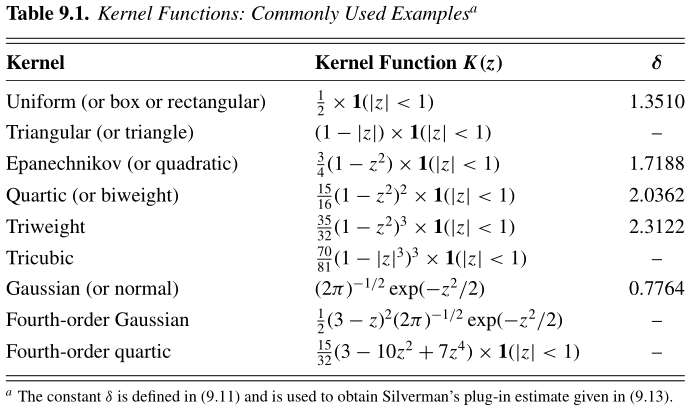
\includegraphics[width=\textwidth]{./resources/CTKernels}
  \label{fig:kernels}
  \end{center}
  \end{figure}
\end{frame}
  
\begin{frame}{Kernel Comparison}
  \begin{figure}[htbp]
  \begin{center}
  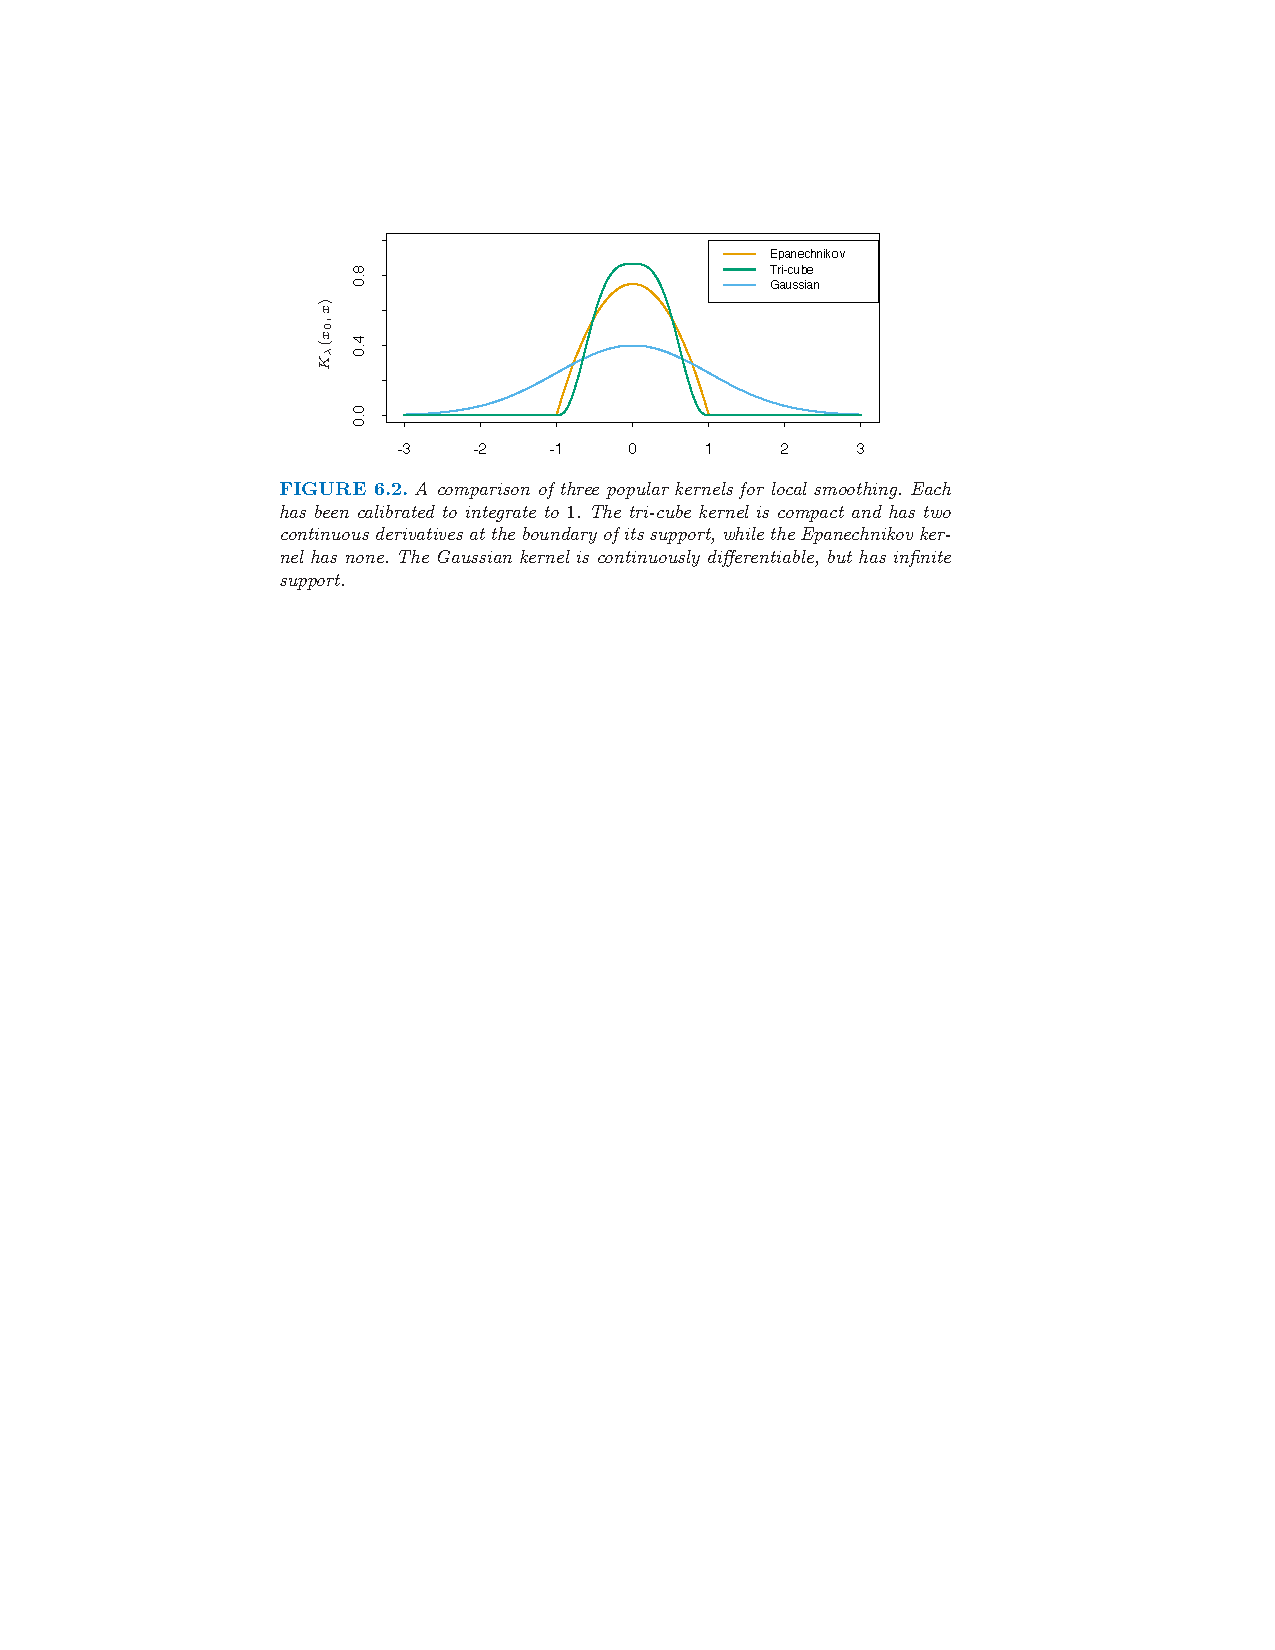
\includegraphics[width=\textwidth]{./resources/kernelfig.pdf}
  \label{kernelfig}
  \end{center}
  \end{figure}
\end{frame}

% from CT 9.3.5%
\begin{frame}{Mean and Variance of $\hat{f}(x_0)$}
  Assume that the derivative of $f(x)$ exists and is bounded, and  $\int z K(z) d z = 0$

  Then the estimator has \textbf{bias}
  \[
    b(x_0) = E \left[\hat{f}(x_0) \right] - f(x_0) = \frac{1}{2} h^2 f''(x_0)\int z^2K(z)dx
  \]

  The \textbf{variance} of the estimator is
  \[
    V \left[\hat{f}(x_0) \right] = \frac{1}{Nh} f(x_0) \int K(z)^2dz \left\{ + o(\frac{1}{Nh}) \right\}
  \]

  So, unsurprisingly, the bias is \textit{increasing} in $h$, and the variance is \textit{decreasing} in $h$.
\end{frame}
 
\begin{frame}{How to Choose $h$}
  \begin{itemize}
    \item We want both bias and variance to be as small as possible, as usual. 
    \item In parametric estimation, it is not a problem: they both go to zero as sample size increases.
    \item In nonparametric estimation reducing $h$ reduces bias, but increases variance; how are we to make his trade off?
    \item Note that how we set $h$ is going to be much more important than the choice of $K(\cdot)$
  \end{itemize}  
\end{frame}

% THIS SECTION FROM GUIDO'S NOTES 
\begin{frame}{Mean Integrated Square Error}
  \begin{itemize}
    \item Start with the \textit{local} performance at $x_0$
    $$ MSE \left[ \hat{f}(x_0) \right] = E \left[ \left( \hat{f}(x_0) - f(x_0) \right)^2 \right] $$
    \item Calculate the \textit{integrated} (as opposed to expected) squared error 
    \begin{align*}
      \int \left( {\hat f}(x)-f(x) \right)^2 dx &=& \int \mbox{bias} ^2 \left( {\hat f}(x) \right) + \mbox{var} \left( {\hat f}(x) \right) dx 
    \end{align*}

  \item Simple approximate expression (symmetric order 2 kernels): $$(\mbox{bias})^2+\mbox{variance}= A
  h^4+B/nh$$
  with $A=\int \left(f''(x)\right)^2 \left(\int u^2K\right)^2 /4$ and $B=f(x)\int K^2$

\end{itemize}  
\end{frame}

%TK Could use Guido's H opt formula here (lecture 16 page 9)
\begin{frame}{Optimal bandwidth}
  \begin{itemize}
  \item The AMISE is $$Ah^4+B/nh$$
  \item Minimize by taking the FOC 
    $$h^*_n=\left(\frac{B}{4An}\right)^{1/5}$$
  
  \item bias and standard error are \emph{both} in $n^{-2/5}$
  \item and the AMISE is $n^{-4/5}$---{\bf not} $1/n$ as it is in parametric models.
  
  \item But: $A$ and $B$ both depend on $K$ (known) and $f(y)$ (unknown), and
  especially ``wiggliness''
  $\int (f'')^2$ (unknown, not easily estimated). Where do we go from here? 
  \end{itemize}
\end{frame}

\begin{frame}{Optimal bandwidth}
  Can be shown that the optimal bandwidth is 
  
  $$h* = \delta \left( \int f''(x_0)^2dx_0\right)^{-0.2}N^{-0.2} $$

  where $\delta$ depends on the kernel used (Silverman 1986) [these $\delta$'s are given in the \href{fig:kernels}{kernel table}]

  Note the "optimal" kernel is Epanechnikov, although the difference is small. 

\end{frame}

\begin{frame}{Silverman's Rule of Thumb}
  \begin{itemize}
  \item If $f$ is normal with variance $\sigma^2$ (may not be a very appropriate benchmark!), the optimal bandwidth
  is
  $$h^*_n=1.06 \sigma n^{-1/5}$$
  \item In practice, typically use \textbf{Silverman's plug-in estimate}:
  $$h^*_n=0.9*\min(s,IQ/1.34)*n^{-1/5}$$ 
  where IQ=interquartile distance
  \item Investigate changing it by a reasonable multiple.
  \end{itemize}
\pause
  This tends to work pretty well. But can we do better? 
\end{frame}

\section{Cross-Validation}

\begin{frame}{Why not search for optimal $h$ in our data?}
  \begin{itemize}
  \item Know we want to minimize MISE. 
  \item One option is to find the $h$ that minimizes it \textit{in sample}
  \begin{itemize}
    \item Loop through increments of $h$
    \item Calculate MISE
  \end{itemize}
  \item Example: Old Faithful R data
  \begin{itemize}
    \item Waiting time between eruptions and the duration of the eruption for the Old Faithful geyser in Yellowstone National Park, Wyoming, USA.
    \item See R code in this folder.
  \end{itemize}
  \end{itemize}
\end{frame}

\begin{frame}{Cross-validation}
  \begin{itemize}
  \item General concept in the whole of nonparametrics: choose $h$ to minimize a criterion $CV(h)$ that approximates
  $$ AMISE(h)=\int E(\hat{f}_n(x)-f(x))^2dx.$$
  \item Usually programmed in metrics software. \emph{If you can do it, do it on a subsample, and rescale.}
  \item CV tries to measure what the expected out of sample (OOS or EPE) prediction error of a new never seen before dataset.
  \item The main consideration is to prevent \alert{overfitting}.
  \begin{itemize}
  \item In sample fit is always going to be maximized by the most complicated model.
  \item OOS fit might be a different story.
  \item ie 1-NN might do really well in-sample, but with a new sample might perform badly.
  \end{itemize}
  \end{itemize}
\end{frame}
  
\begin{frame}{Sample Splitting/Holdout Method and CV}
  Cross Validation is actually a more complicated version of \alert{sample splitting} that is one of the organizing principles in machine learning literature.
  
  \begin{description}
  \item[Training Set] This is where you estimate parameter values.
  \item[Validation Set] This is where you choose a model- a bandwidth $h$ or tuning parameter $\lambda$ by computing the error.
  \item[Test Set] You are only allowed to look at this after you have chosen a model. \alert{Only Test Once}: compute the error again on fresh data.
  \end{description}
  \begin{itemize}
  \item Conventional approach is to allocate 50-80\% to training and 10-20\% to Validation and Test.
  \item Sometimes we don't have enough data to do this reliably.
  \end{itemize}
  \end{frame}
  
\begin{frame}{Sample Splitting/Holdout Method}
  \begin{center}
  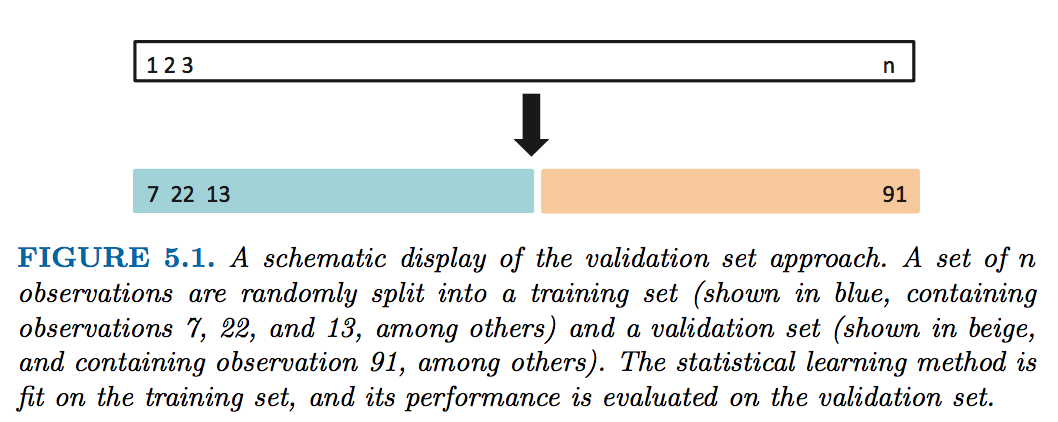
\includegraphics[width=\textwidth]{./resources/split-sample}
  \end{center}
\end{frame}
  
\begin{frame}{Challenge with Sample Splitting}
  \begin{center}
  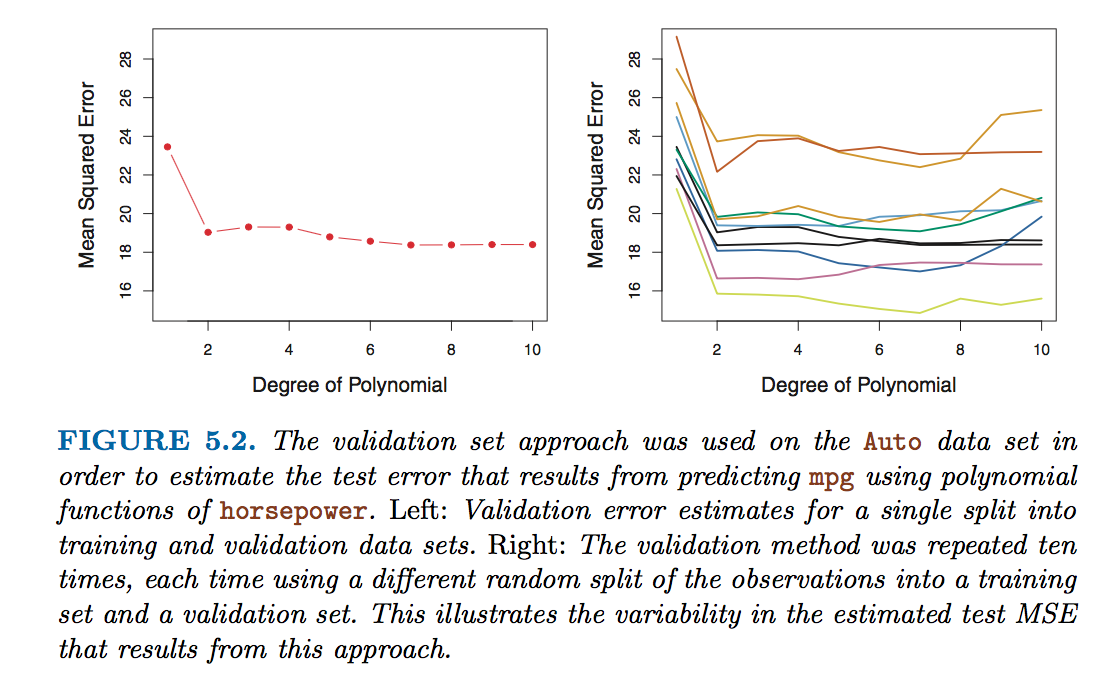
\includegraphics[width=\textwidth]{./resources/validation-10fold}
  \end{center}
\end{frame}
  
\begin{frame}{$k$-fold Cross Validation}
  \begin{itemize}
  \item Break the dataset into $k$ equally sized ``folds'' (at random).
  \item Withhold $i=1$ fold
  \begin{itemize}
  \item Estimate the model parameters $\hat{\theta}^{(-i)}$ on the remaining $k-1$ folds
  \item Predict $\hat{y}^{(-i)}$ using $\hat{\theta}^{(-i)}$ estimates for the $i$th fold (withheld data).
  \item Compute $MSE_i =\frac{1}{k \cdot N} \sum_j (y^{(-i)}_j -\hat{y}^{(-i)}_j)^2$.
  \item Repeat for $i=1,\ldots,k$.
  \end{itemize}
  \item Construct $\widehat{MSE}_{k,CV} = \frac{1}{k} \sum_i MSE_{i}$
  \end{itemize}
\end{frame}
  
\begin{frame}{$k$-fold Cross Validation}
  \begin{center}
  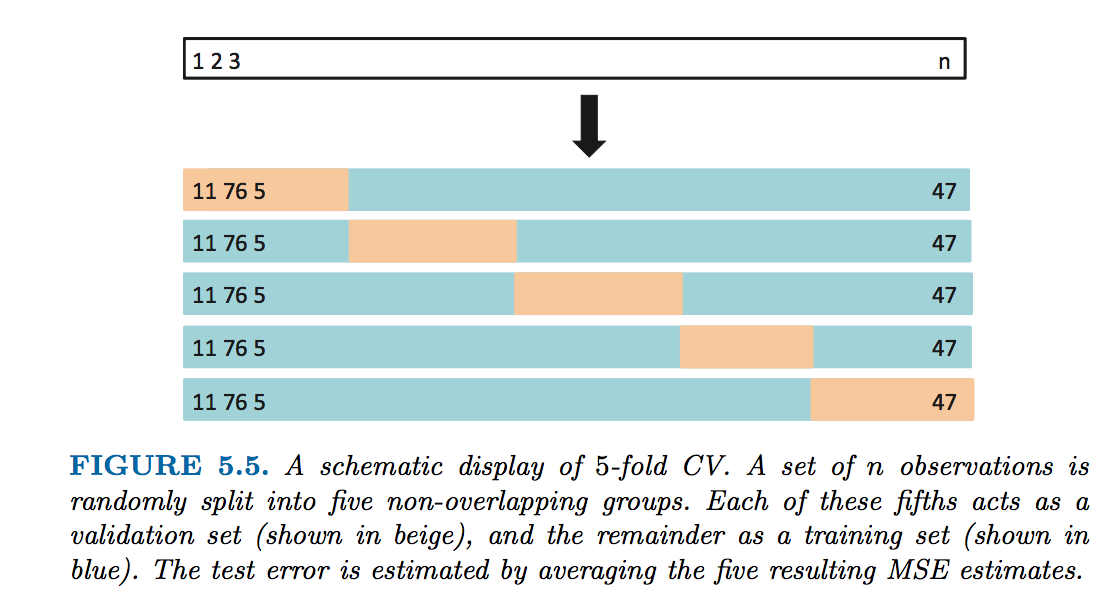
\includegraphics[width=\textwidth]{./resources/split-cv5}
  \end{center}
\end{frame}

\begin{frame}{Leave One Out Cross Validation (LOOCV)}
  Same as $k$-fold but with $k=N$.
  \begin{itemize}
  \item Withhold a single observation $i$
  \item Estimate $\hat{\theta}_{(-i)}$.
  \item Predict $\hat{y}_i$ using $\hat{\theta}^{(-i)}$ estimates
  \item Compute $MSE_i =\frac{1}{N} \sum_j (y_i -\hat{y}_i(\hat{\theta}^{(-i)}))^2$.
  \end{itemize}
  \vspace{0.2cm}
  Note: this requires estimating the model $N$ times which can be costly.
\end{frame}
    
\begin{frame}{LOOCV vs $k$-fold CV}
  \begin{center}
  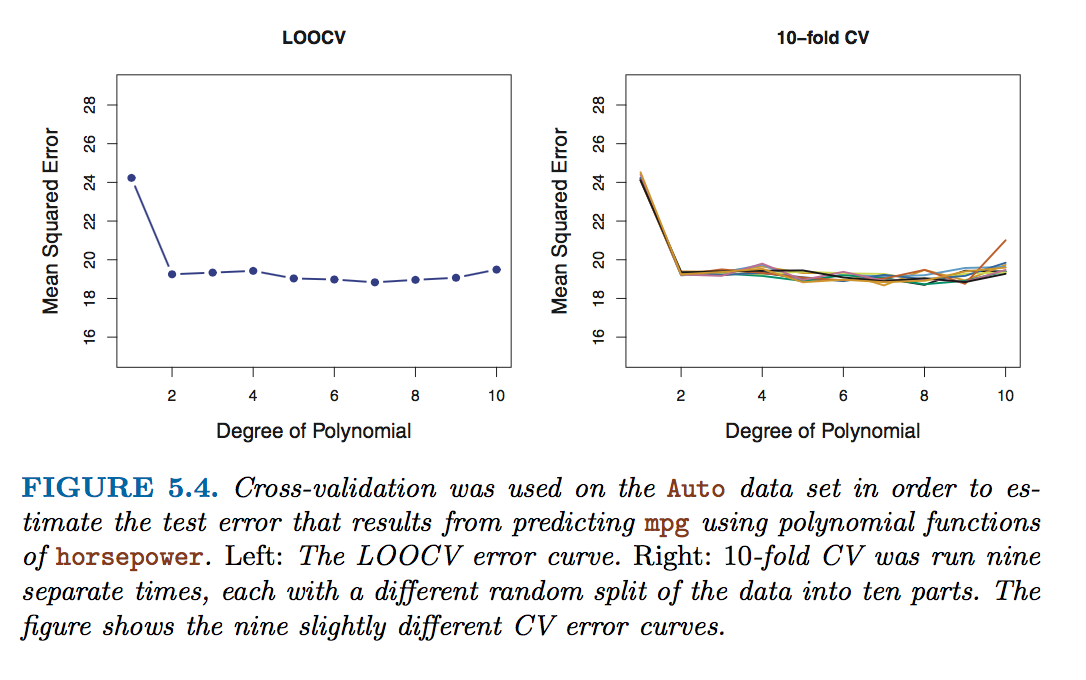
\includegraphics[width=\textwidth]{./resources/comparison-cv}
  \end{center}
\end{frame}
  
\begin{frame}{Cross Validation}
  \begin{itemize}
  \item Main advantage of cross validation is that we use all of the data in both \alert{estimation} and in \alert{validation}.
  \begin{itemize}
  \item For our purposes validation is mostly about choosing the right bandwidth or tuning parameter.
  \end{itemize}
  \item We have much lower variance in our estimate of the OOS mean squared error.
  \begin{itemize}
  \item Hopefully our bandwidth choice doesn't depend on randomness of splitting sample.
  \end{itemize}
  \end{itemize}
\end{frame}
  
  
\begin{frame}{Test Data}
  \begin{itemize}
  \item In Statistics/Machine learning there is a tradition to withhold 10\% of the data as \alert{Test Data}.
  \item This is \alert{completely new data} that was not used in the CV procedure.
  \item The idea is to report the results using this test data because it most accurately simulates true OOS performance.
  \item We don't do much of this in economics.\\
   (Should we do more?)
  \end{itemize}
\end{frame}


\frame{\frametitle{Local Bandwidths}

\pause

If you only care about $f(y)$ at some given point, then 
\[
A=f''(y)^2 \left(\int u^2K\right)^2/4 \mbox{ and } B=f(y)\int K^2.
\]

\pause

So in a low-density region, worry about variance and take $h$ larger.
In a curvy region, worry about bias and take $h$ small.
 
}

\frame{\frametitle{Higher-Order Kernels}
\begin{itemize}
\item $K$ of order $r$ iff $\int x^j K(x) dx=0$ for $j<r$ and $\int x^r
K(x)dx \neq 0$. Try $r>2$?
\item The beauty of it: bias in $h^r$ if $f$ is at least $C^r$\ldots so AMISE can be
reduced to $n^{-r/(2r+1)}$, almost $\sqrt{n}$-consistent if $r$ is
large. 
\item But gives wiggly (and sometimes negative) estimates
$\rightarrow$ leave them to theorists. 
\end{itemize}
}

\frame{\frametitle{Back to the CDF}

Since now we have estimated the density with
$${\hat f}_n(x)= \frac{1}{nh}\sum_{i=1}^n K\left(
\frac{x-x_i}{h}\right),$$
\pause
a natural idea is to integrate; let $\mathcal{K}(x)=\int_{-\infty}^x K(t)dt$, try

$$ {\hat F}_n(y)= \frac{1}{n}\sum_{i=1}^n \mathcal{K}\left(
\frac{y-y_i}{h}\right) $$
as a reasonable estimator of the cdf in $y$.

\pause

Very reasonable indeed:
\begin{itemize}
  \item when $n \longrightarrow \infty$ and $h$ goes to zero (at rate
    $n^{-1/3}$\ldots) 
      it is consistent at rate $\sqrt{n}$
  \item it is nicely smooth
  \item by construction it accords well with the density estimator
  \item \ldots\ it is a much better choice than the empirical cdf.
\end{itemize}

}

\section{Example: Auctions}

\begin{frame}{Example application: Auctions}
  \begin{itemize}
    \item Why auctions? 
    \item Great introduction to structural approach. Arguably the most successful application. 
    \item Auctions are an example of a game with assymetric information: participants know the primitives of the game, but do not know their rivals exact valuations. 
    \item By imposing rationality/ profit maximization, we can recover the distribution of values. 
    \item Can then run counterfatuals
    \item Example: Asker (AER 2008) - stamp cartel 
\end{itemize}

For more detail, check out Chris Conlon's slides in this folder, or John Asker's PhD \href{http://www.johnasker.com}{lecture notes}.

% http://www.johnasker.com/Auctions%20I.pdf
\end{frame}

\begin{frame}{Setup}
Let's consider the first price sealed bid (FPSB) auction

\begin{itemize}
  \item bidders have \textbf{private information} (or type) scalar rv $X_i$ with realization $x_i$
  \item signals are informative: $dE[U|x]/dx >0$ 
  \item given their signal, they make a bid $b_i$
  \item if its the highest bid, recieve utility $[U| x_i,x_{-i}] - b_i$ 
  \item else get $0$
  \item note that if we assume values are \textbf{independent}, we get $E[U| x_i,x_{-i}]=E[U | x_i]$
\end{itemize}

This introduces a tradeoff in first price auctions: Increasing the bid increases the probability of winning; but reduces your net utility from the object.

\end{frame}

\begin{frame}{How to bid?}

Denote the equilibrium bid as $B_i$, with realizations $b_i$

\vspace{10pt}

Perfect Bayes Nash equilibrium:
\vspace{-10pt}

\begin{multline*} 
  max_{\tilde b}  \left( E \left[ U_i | X_i = x_i \right] - b , max_{j \in N_{-i}} B_j \leq \tilde b \right) \\ Pr \left( max_{j \in N_{-i}} B_j \leq \tilde b | X_i = x_i \right) 
\end{multline*}

See Athey and Haile or Krishna for an accessible derivation. 

\end{frame}  

\begin{frame}{Can find bid as a function of primitives}

  $$ v(x_i,\mathbf{x_i};N) = b_i + \frac{G_{M_i | B_i} \left(b_i | b_i ; N \right)}{ g_{M_i | B_i} \left(b_i | b_i ; N \right)} $$

  where $G_{M_i | B_i}$ and $g_{M_i | B_i}$ are the CDF and PDF of the max bids given $b_i$ and $N$ 

  \begin{itemize}
    \item we are typically interested in the LHS
    \item RHS is stuff we can observe or compute
    \item nice linear structure makes this easy to work with
    \item Guerre, Perrigne and Vuong (2000): can leverage assumption of equilibrium best response and invertibility of $b$ to recover $v$
  \end{itemize}

\end{frame}  

\begin{frame}[allowframebreaks]{Estimation strategy}
  [Assumption: FPSB with symmetric IPV]

  \begin{enumerate}
    \item Leverage independence assumption: 
    \begin{align*}  
      G_{M_i | B_i}(m_i | b_i; N) &= G_{M_I | n} \\
                                  &= Pr(max_{j\neq i} B_j \leq m_i | n )      
    \end{align*}  
    \item Value equation becomes 
    $$ u = b + \frac{G_B \left(b | n \right)}{ (n-1) g_B \left(b | n \right)} $$
    where $G_B$ and $g_B$ are now the marginal distribution of equilibrium bids and the densities in $n$ bidder auctions

    \framebreak
    
    \item can estimate $G$ and $g$ using kernels 


    \item now have 
    $$ \hat u = b + \frac{\hat G_B \left(b | n \right)}{ (n-1) \hat g_B \left(b | n \right)} $$

    \item finally, can recover the distribution of values with another kernel 
    
    \begin{eqnarray*}
      \hat{f}(u) = \frac{1}{T_nh_f} \sum_{T=1}\frac{1}{n_t}\sum_{i=1}^{n}  K \left( \frac{u_i - \hat u_{it}}{h_f} \right)
    \end{eqnarray*}

  \end{enumerate}

\end{frame}  

\begin{frame}{Algoritm}
\begin{itemize}
   \item for each $b_o$, estimate $\hat G_B(b_0|n)$ and $\hat g_B(b_0|n)$ using \textbf{all the data}
   \item infer $\hat u(b_0)$
   \item estimate $\hat f$ 
   \item plot bids, adjust bandwidth etc 
   \item run counterfactuals 
\end{itemize}
\end{frame}

\section{Non-parametric Regression}

\begin{frame}{Nonparametric Regression}
  \begin{itemize}
  \item Often we're interested in $E\left[Y_i | X_i = x \right]$ 
  \item If $X$ is discrete, can just average for each value
  \item But often times we want to smooth across values of $X$
  \begin{itemize}
    \item Each bin could have small $n$. [Likely if $X$ has many dimensions]
    \item $X$ could be continuous  
  \end{itemize}
  \item One option is to pick a parametric functional form $y=f(x)$. But often hard to think about how sensible these assumptions are (and what they impose on the economics of the problem)
  \item An alternative is to extend the concepts of nonparametric density estimation
  \end{itemize}
\end{frame}

\begin{frame}{A Fake Data Example}
HTF 2.3 includes an example classification problem. 

An (unknown) model maps a pair of inputs $X_1$ and $X_2$ into classes of either BLUE or ORANGE. 

Training data: 
Imagine we have 100 points from each class. 

OLS solution 
\begin{eqnarray*}
Y=&ORANGE \mbox{ if } Y* = x^T\hat \beta &> 0.5 \\
Y=&BLUE  \mbox{ if }   Y* =  x^T\hat \beta &\leq 0.5
\end{eqnarray*}
\end{frame}


\begin{frame}{Linear Probability Model}
  \vspace{-15pt}
    
  \begin{figure}[htbp]
  \begin{center}
  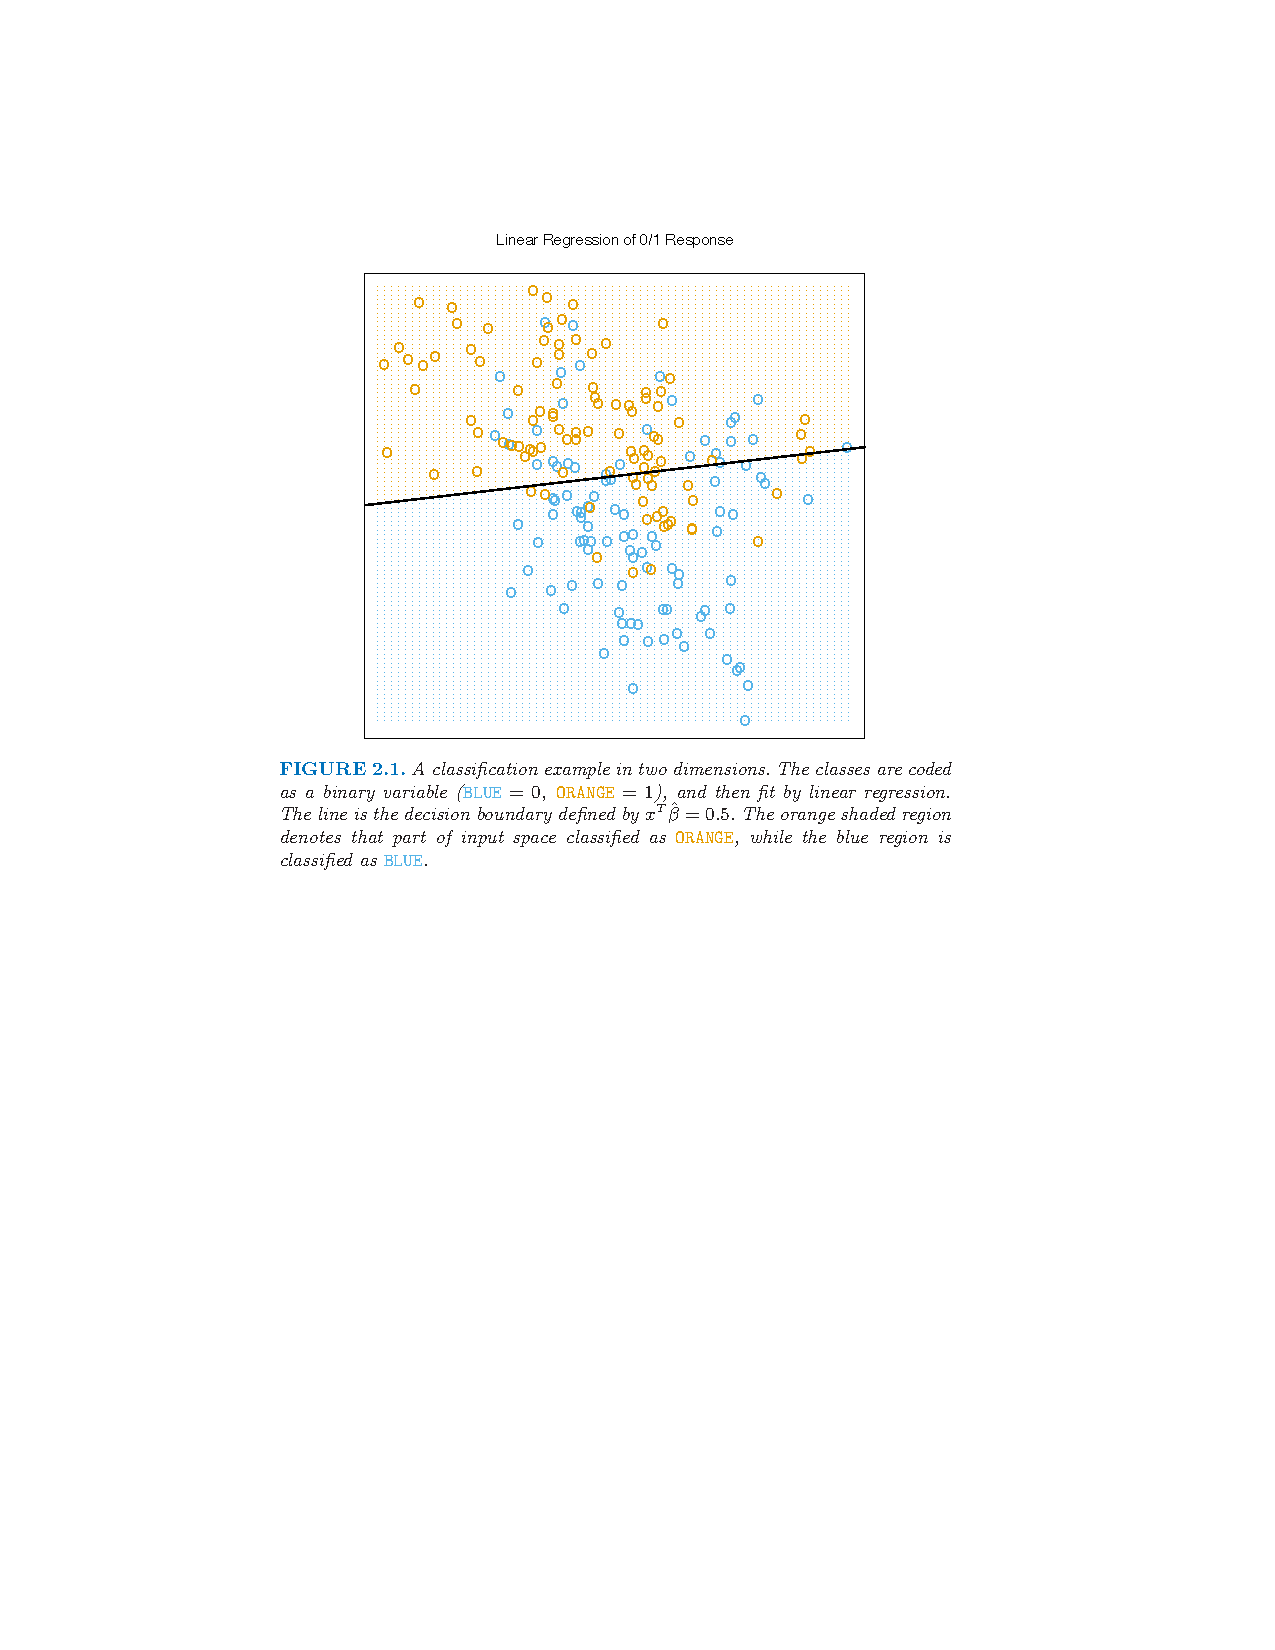
\includegraphics[height = .95\textheight]{./resources/classifierOLS.pdf}
  \label{classOLS}
  \end{center}
  \end{figure}
\end{frame}

\begin{frame}{Is this the best we can do?}

Consider two DGPs: 
\begin{enumerate}
  \item Draws from bivariate normal distribution with uncorrelated components but different means (2 overlapping types)
  \item Mixture of 10 low variance (nearly point mass) normal distributions where the individual means were drawn from another normal distribution. (10 nearly distinct types).
\end{enumerate}

In the case of 1, OLS is the best we can do. 

In the case of 2, OLS will perform very poorly.

\end{frame}

\begin{frame}{Alternative}
\begin{itemize}
\item Lots of potential alternatives to our decision rule.
\item A simple idea is to hold a majority vote of neighboring points 
\begin{eqnarray*}
Y^{*} = \frac{1}{k} \sum_{x_{-i} \in N_k(x)} y_i
\end{eqnarray*}
\item How many parameters does this model have: None? One? $k$? 
\item Technically it has something like $N/k$.
\item As $N \rightarrow \infty$ this means we have an infinite number of parameters! (This is a defining characteristic of non-parametrics).
\end{itemize}
\end{frame}

\begin{frame}{15 Nearest Neighbor}
  \vspace{-15pt}
\begin{figure}[htbp]
\begin{center}
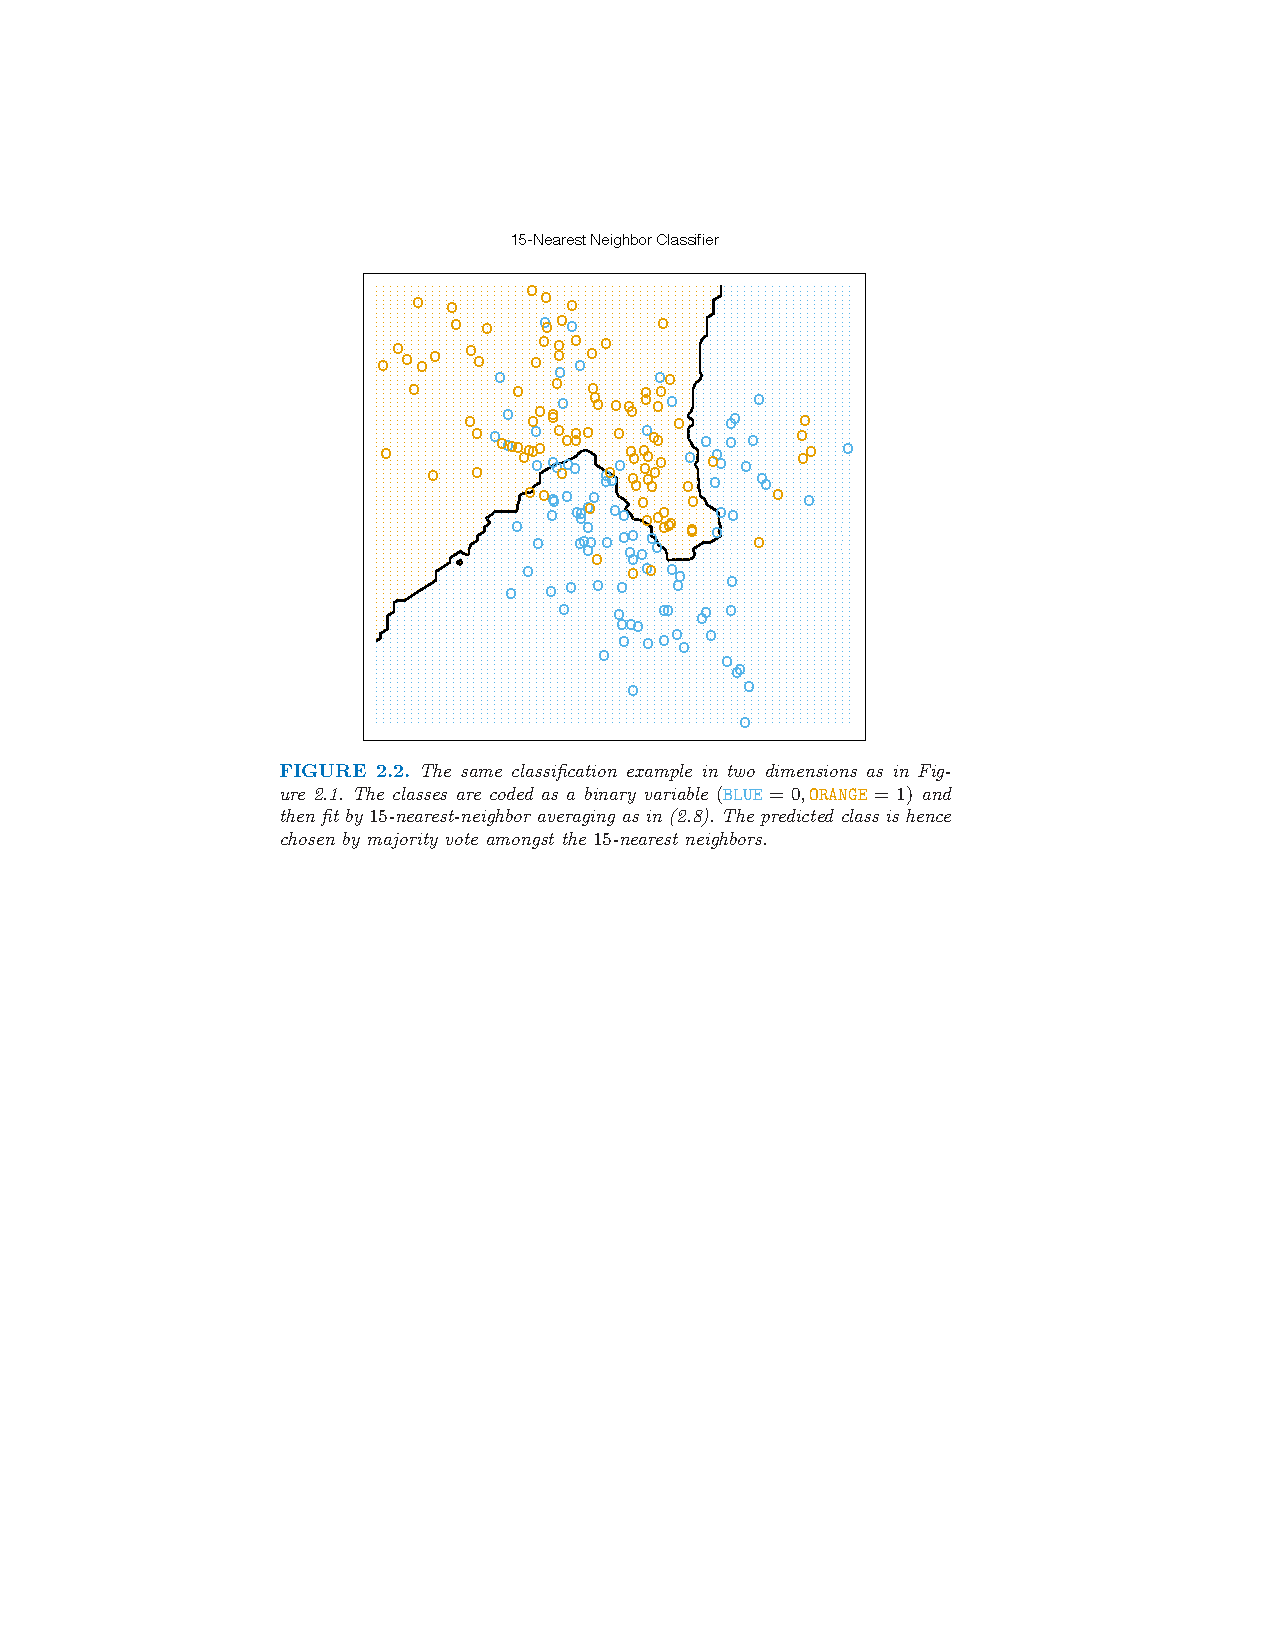
\includegraphics[width=3.5in]{./resources/classifier15nn.pdf}
\label{class15nn}
\end{center}
\end{figure}
\end{frame}

\begin{frame}{Extreme: 1 Nearest Neighbor}
\vspace{-15pt}

\begin{figure}[htbp]
\begin{center}
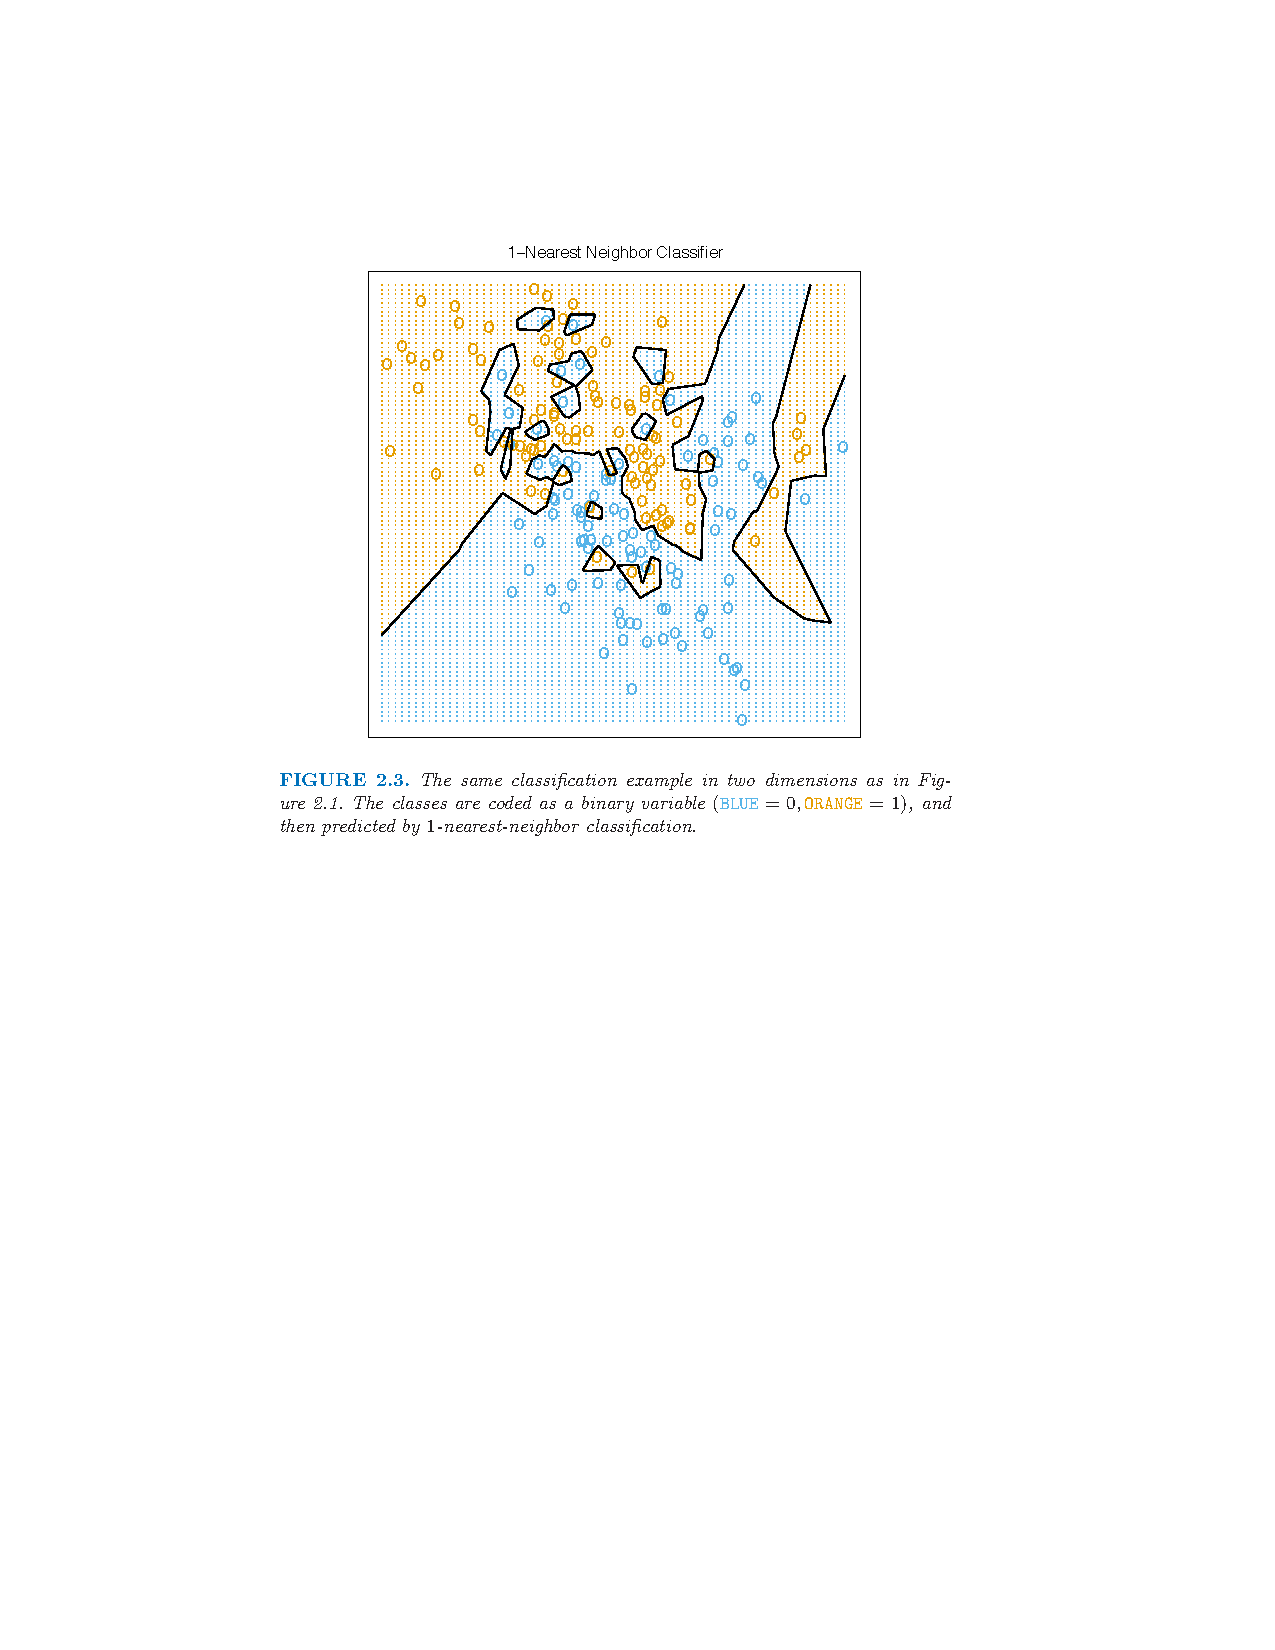
\includegraphics[width=3.5in]{./resources/classifier1nn.pdf}
\label{class15nn}
\end{center}
\end{figure}
\end{frame}

\begin{comment}
\begin{frame}{Comparisons}
  \begin{itemize}
  \item What would happen if $K \rightarrow N$?
  \item The k-NN model is locally constant.
  \item The k-NN approach tends to be really bumpy which can be undesirable.
  \item The OLS model is globally linear (is this always true?)
  \end{itemize}
  \end{frame}
  \begin{frame}{What about?}
  \begin{itemize}
  \item If we fixed the fact that there are discrete jumps in who is in the neighborhood by smoothly weighting observations and varying those weights instead (Kernels).
  \item Another drawback of $k-NN$ is that we consider distance in each $X$ dimension on the same scale, perhaps we could rescale the data to improve our ``closeness'' measure.
  \item Instead of fitting a constant locally, we fit a linear function locally (Lowess).
  \item Instead of using a global linear approximation in OLS use a more flexible nonlinear one.
  \item There is a bias/variance tradeoff. \alert{explain}.
  \end{itemize}
\end{frame}
\end{comment}

\begin{frame}{Bias Variance Decomposition}
We can decompose any estimator into two components
\begin{eqnarray*}
\underbrace{E[(y- \hat{f}(x))^2]}_{MSE} =\underbrace{\left( E[\hat{f}(x) - f(x)] \right)^2}_{Bias^2}  +  \underbrace{E \left[ \left(\hat{f}(x) - E[\hat{f}(x) \right] \right)^2}_{Variance} 
\end{eqnarray*}
\begin{itemize}
\item In general we face a tradeoff between bias and variance.
\item In k-NN as $k$ gets large we reduce the variance (each point has less influence) but we increase the bias since we start incorporating far away and potentially irrelevant information.
\item In OLS we minimize the variance among unbiased estimators assuming that the true $f$ is linear and using the entire dataset. 
\end{itemize}
\end{frame}


\begin{frame}{Big Data}
  \begin{itemize}
  \item It used to be that if you had $N=50$ observations then you had a lot of data.
  \item Those were the days of finite-sample adjusted t-statistics.
  \item Now we frequently have 1 million observations or more, why can't we use k-NN type methods everywhere?
  \end{itemize}
\end{frame}
  
\begin{frame}{Curse of Dimensionality}
  Take a unit hypercube in dimension $p$ and we put another hypercube within it that captures a fraction of the observations $r$ within the cube
  \begin{itemize}
  \item Since it corresponds to a fraction of the unit volume, $r$ each edge  will be $e_p(r) = r^{1/p}$.
  \item $e_{10}(0.01) = 0.63$ and $e_{10}(0.1) = 0.80$, so we need almost 80\% of the data to cover 10\% of the sample!
  \item If we choose a smaller $r$ (include less in our average) we increase variance quite a bit without really reducing the required interval length substantially.
  \end{itemize}
\end{frame}
  
\begin{frame}{Curse of Dimensionality}
  \begin{figure}[htbp]
  \begin{center}
  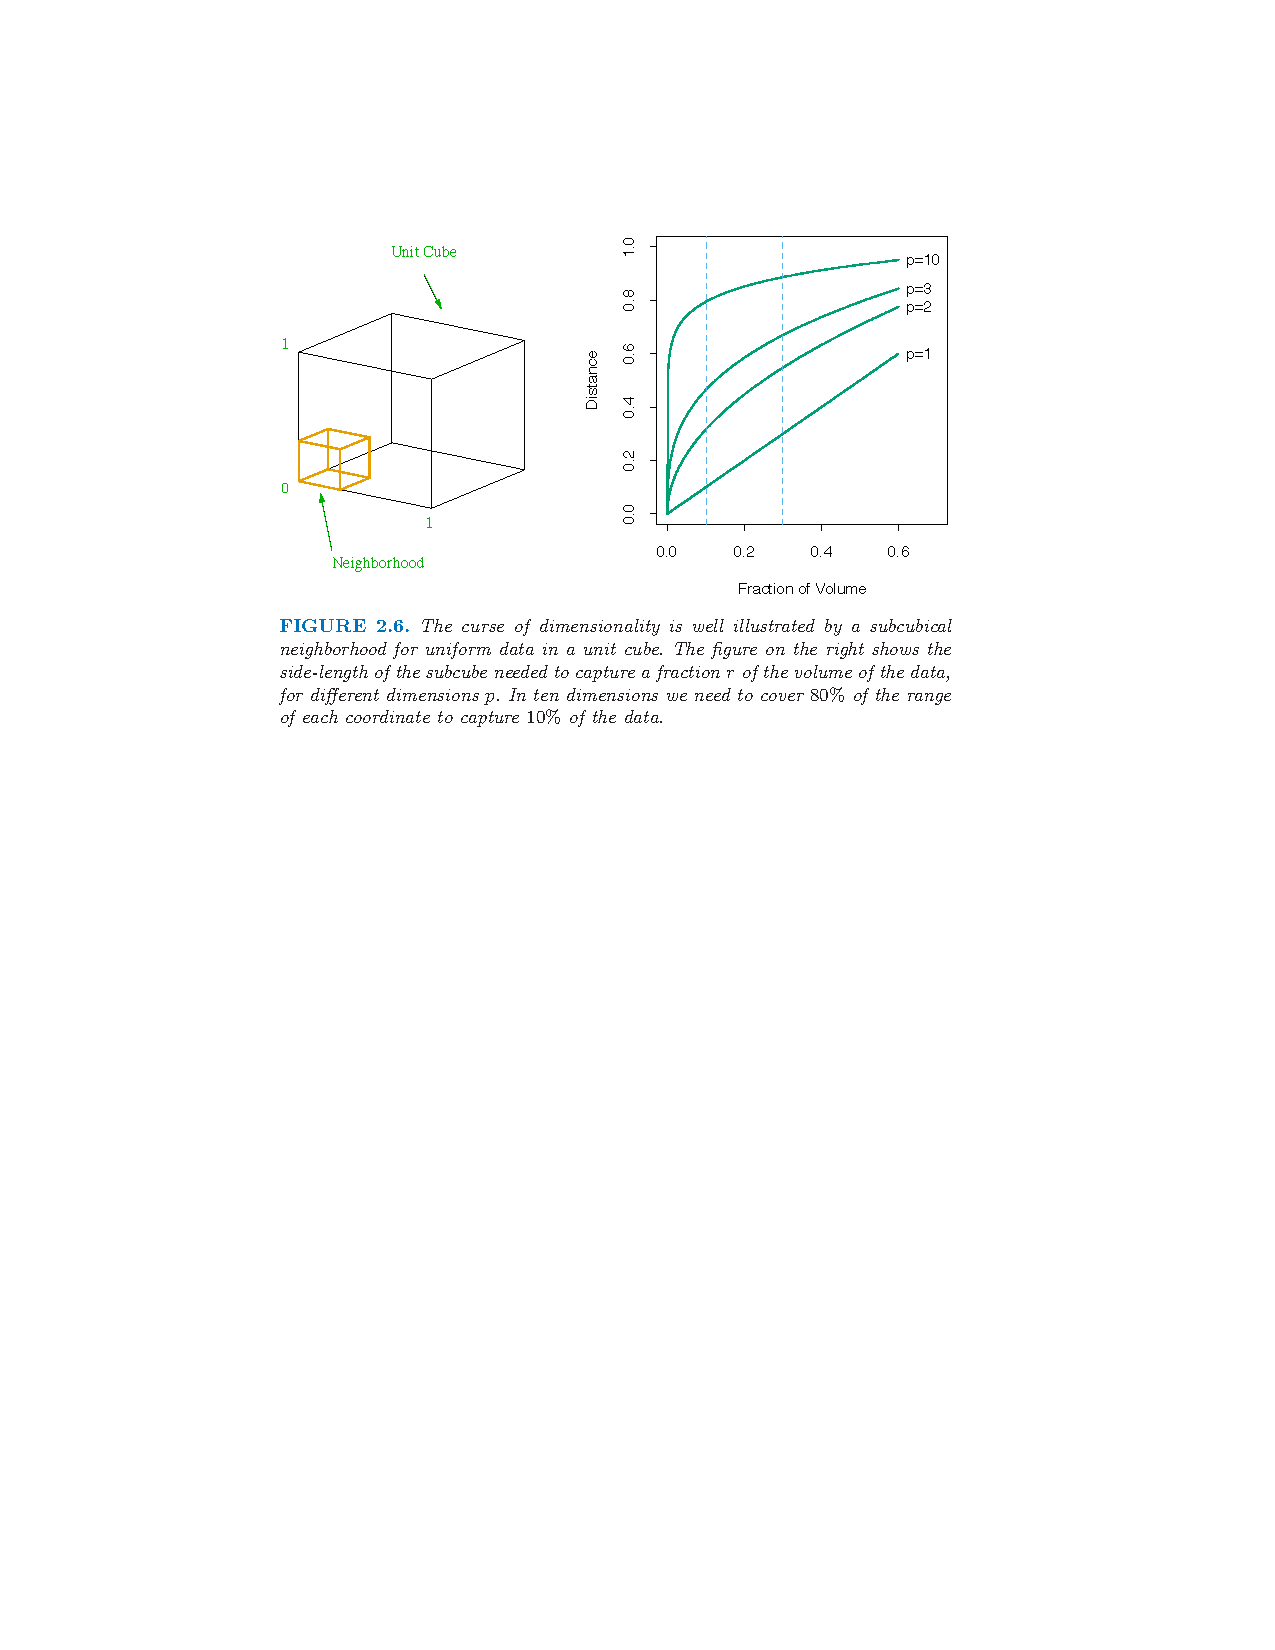
\includegraphics[width=\textwidth]{./resources/figure26.pdf}
  \label{class15nn}
  \end{center}
  \end{figure}
\end{frame}
  
\begin{frame}{Curse of Dimensionality}
  Don't worry, it only gets worse:
  \begin{eqnarray*}
  d(p,N) = \left(1-\left(\frac{1}{2} \right)^{1/N} \right)^{1/p}
  \end{eqnarray*}
  
  \begin{itemize}
  \item $d(p,N)$ is the distance from the origin to the closest point.
  \item $N=500$ and $p=10$ means $d = 0.52$ or that the closest point is closer to the boundary than the origin!
  \item Why is this a problem?
  \item In some dimension nearly every point is the closest point to the boundary -- when we average over nearest neighbors we are \alert{extrapolating} not \alert{interpolating}.
  \end{itemize}
\end{frame}
  
\begin{frame}{Back to Bias - Variance}
What minimizes MSE?
\begin{eqnarray*}
f(x_i) = E[Y_i | X_i] 
\end{eqnarray*}
\begin{itemize}
\item Seems simple enough (but we are back where we started).
\item How do we compute the expectation ?
\item k-NN tries to use local information to estimate conditional mean
\item OLS uses entire dataset and adds structure $ y = x \beta$ to the problem.
\item A natural middleground point is to use a smoother that weights "close" observations more than "far" ones. 
\end{itemize}
\end{frame}

\begin{frame}{Common weights}
  Consider the following \textbf{local weighted average estimator}: 
   $$ \hat m(x_0) = \sum_{i=1}^{N} w_{i0,h}y_i$$

   where $w_{i0,h} = w(x_i,x_0,h)$ and $\sum_i  w_{i0,h} = 1$. 

\pause 

  Rearranging, can see that OLS uses the following weights

  $$ \hat m_{OLS}(x_0) = \sum_{i=1}^{N} \lbrace \frac{1}{N} + \frac{ (x_0 - \bar{x}) (x_i - \bar{x})}{\sum_j (x_j - \bar{x})^2} \rbrace y_i $$

  CT note that these weights can actually \textit{increase} with the distance between $x_0$ and $x_i$! 
  (for example if $x_i > x_0 > \bar{x}$ )
  
\end{frame}

\begin{frame}{k-NN is simply a running average}
  $$ \hat m_k(x_0) = \frac{1}{k}(y_{i-(k-1)/2} + ... + y_{i+(k-1)/2}$$

  Can immediately see that this will not be great at the end points. 
  
  For the smallest and largest $x$, the average is one sided. This is the \textbf{boundary problem}. 

\end{frame}

\begin{comment}
\begin{frame}{Link to density estimation}
  CT  
  
\end{frame}
\end{comment}

\begin{frame}{Nonparametric Regression}
Of course, we could also average all the observations within some bandwidth $h$  


Nadaraya-Watson:
\[
{\hat m}_n(x)=\frac{\sum_{i=1}^n y_i
K\left(\frac{x-x_i}{h}\right)}{\sum_{i=1}^n
K\left(\frac{x-x_i}{h}\right)}.
\]

where $K(\cdot)$ is a kernel weighting function as above. 

Again, bias in $h^2$ and variance in $1/nh$ if $p_x=1$.

\end{frame}

% COULD PLUG IN GUIDOS DESCRIPTION HERE 

\begin{frame}{Choosing $h$}
Plug-in estimates work badly here. 

In most cases leave one out cross-validation is feasible

Can be shown that this amounts to 
$$ \min_h CV(h) = \sum_{i=1}^N \left(\frac{y_i - \hat m (x_i)}{1 - \left[w_{ii,h}/\sum_j w{ji,h}\right]} \right)^2 $$

So not that hard: for each $h$, only need to compute one weighted average $\hat m(x_i)$ for each $N$.
\end{frame}

\subsection{Multivariate Kernels}
\begin{frame}{Multivariate Kernels}
  Typically we are interested in more than one regressor 
  $$ y_i = m(x_{1i},...,x_{ki}) $$

  the NW kernel estimator extends naturally to $k$ dimensions

  \[
{\hat m}(\mathbf{x_0})=\frac{\sum_{i=1}^N y_i
K\left(\frac{\mathbf{x_1}-\mathbf{x_0}}{h}\right)}{\sum_{i=1}^N
K\left(\frac{\mathbf{x_1}-\mathbf{x_0}}{h}\right)}.
\]
 where we just use a mutivariate kernel. 

 If you rescale by dividing by the standard deviation, you can even use a common bandwidth. 

\end{frame}

\begin{comment} 
\begin{frame}{Density/Distribution Estimation}
  One of the more successful and popular uses of nonparametric methods is estimating the density or distribution function $f(x)$ or $F(x)$.
  \begin{itemize}
  \item Estimating the CDF is easy and something you have already done
  \item Q-Q plots, etc.
  \end{itemize}
  \begin{eqnarray*}
  \hat{F}_{ECDF}(x_0) = \frac{1}{N} \sum_{i=1}^N (x_i \leq x_0 )
  \end{eqnarray*}
  \begin{itemize}
  \item Differentiating to get density is unhelpful : $F_{ECDF}'(x) = 0$ in most places.
  \end{itemize}
  \end{frame}
  
  \frame{\frametitle{What if $y$ is of dimension $p_y>1$?}
  
  \pause
  
  ``Easy'': use $p_y$-dimensional $K$ (often a $p_y$-product of 1-dim
  kernels) and bandwidth $h$, and do
  
  \pause
    
  \[
  {\hat f}_n(y)= \frac{1}{nh^p_y}\sum_{i=1}^n K\left(
  \frac{y-y_i}{h}\right).
  \]
  
  \begin{itemize}
  \item {\bf 1st minor pitfall:} the various dimensions may have very
  different variances, so use  $(h_1,\ldots,h_{p_y})$.
  \item {\bf 2nd minor pitfall:} they may be strongly correlated; then
  sphericize first.
  \item {\bf Major problem:} next slide\ldots
  \end{itemize}
   }
  
  \frame{\frametitle{The Curse of Dimensionality}
  \pause
  
  \begin{itemize}
  \item Computational cost increases exponentially.
  \item {\em Much worse:} to achieve precision $\epsilon$ in dimension $p_y$, the number of
    observations you need increases as
  \[
  n \simeq \epsilon^{-(2+p_y/2)}.
  \]
  \item The {\em empty space\/} phenomenon: 
  if $(y_1,\ldots,y_{p_y})$ all are iid uniform on $[-1,1]$, then only
  $n/(10^{p_y})$ observations on average have all components in
  $[-0.1,0.1]$. Bias still in $h^2$, but variance in $1/nh^{p_y}$ now.
  \end{itemize}
  }
\end{comment}

\frame{\frametitle{Silverman's Table}
   Silverman (1986 book) 
  provides a table illustrating the difficulty of kernel estimation
  in high dimensions. To estimate the density at 0 of a $N(0,1)$ with
  a given accuracy, he reports:
  
  \begin{table}
  \begin{center}
  \vspace{1ex}
  \begin{tabular}{|c|c|}\hline
  Dimensionality Required & Sample Size    \\
  \hline
  1               &  4    \\
  2               &  19    \\
  5           & 786 \\
  7          & 10,700 \\
  10           & 842,000 \\
  \hline
  \end{tabular}
  \end{center}
  \end{table}
  
  \pause
  
  {\bf Not to be taken lightly\ldots} in any case convergence  with
  the optimal bandwidth  is in $n^{-2/(4+p_y)}$ now---and Silverman's
  rule of thumb for choosing $h^*_n$ must be adapted too. }

\begin{comment}
\frame{\frametitle{Usually we care about conditional densities}
  
  \pause
  
  That is: we have covariates $x$, we want the density $f(y|x)$. Again, ``easy'':
  
  \pause
  
  \begin{enumerate}
  \item get a kernel estimator of the joint density $f(y,x)$;
  \item and one of of the marginal density $f(x)$;
  \item then define
  \[
  \hat{f}_n(y|x)=\frac{\hat{f}_n(y,x)}{\hat{f}_n(x)}=\frac{\frac{1}{n
  h_y^{p_y}h_x^{p_x}}\sum_{i=1}^n
  K\left(\frac{y-y_i}{h_y}\right)K\left(\frac{x-x_i}{h_x}\right)}{\frac{1}{h_y^{p_y}}
  \sum_{i=1}^n K\left(\frac{x-x_i}{h_x}\right)}.
  \]
  \end{enumerate}
  
  \pause
  
  But the joint density is $(p_x+p_y)$ dimensional\ldots\ and the curse
  strikes big time.
}
\end{comment}

\subsection{Local linear}
\begin{frame}[allowframebreaks]{Back to one dimesion}
We can interpret the standard kernel estimator as estimating a constant regressino function $g(x) = m$ 

where $$\hat m = \mbox{arg min}_{m_0} \sum_{i=1}^{N} K \left( \frac{x_i - x_0}{h} \right) \cdot \left( y_i - m_0 \right)^2 $$

Taking the FOC, we see that this yields 

$$\hat g(x) = \hat m = \sum_{i=1}^{N} K \left( \frac{x_i - x_0}{h} \right) \cdot y_i / \sum_{i=1}^{N} K \left( \frac{x_i - x_0}{h} \right) $$

\end{frame}

\begin{frame}[allowframebreaks]{Local Linear Regression}

This suggests other functions instead of constants (that is why we're interested in this regression in the first place!)

A natural option is \textbf{local linear regression}:
$$ m(x) = \alpha + \beta(x-x_0) $$ 

where $$(\hat \alpha, \hat \beta) = \mbox{arg min}_{m_0} \sum_{i=1}^{N} K \left( \frac{x_i - x_0}{h} \right) \cdot \left( y_i - \alpha + \beta(x_i-x_0) \right)^2 $$

\framebreak

Advantages:
\begin{itemize}
\item the bias becomes 0 if the true $m(x)$ is linear.
\item the coefficient of $(x-x_i)$ estimates $m'(x)$.
\item behaves better in ``almost empty'' regions.
\end{itemize}
{Disadvantages:} hardly any, just do it! How? 

\pause 

Locally Weighted Scatterplot Smoothing (\textbf{lowess})
\begin{itemize}
  \item uses a variable bandwidth $h_{0,k}$ 
  \item tricubic kernel 
  \item downweights observations with large residuals (through $N$ iterations)
  \item Output: robust to outliers, smooth, and better at boundaries
  \item In most packages, but can be 
\end{itemize}

\end{frame} 

\begin{frame}{Example from Cameron and Trivedi}
  \begin{figure}[htbp]
  \begin{center}
  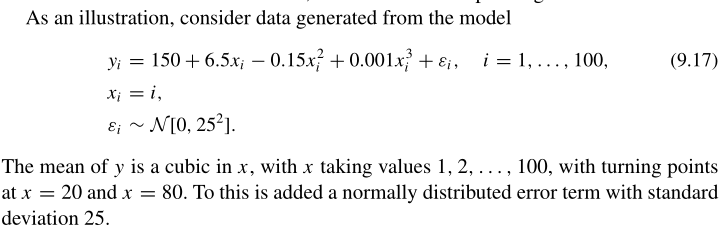
\includegraphics[width=\textwidth]{./resources/CTsimulation}
  \label{loclinear1}
  \end{center}
  \end{figure}
  \end{frame}
  
\begin{frame}{k-NN performance}
  \begin{figure}[htbp]
  \begin{center}
  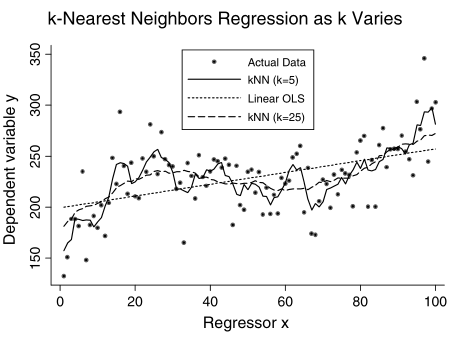
\includegraphics[width=\textwidth]{./resources/CTknn}
  \label{loclinear2}
  \end{center}
  \end{figure}
\end{frame}
    
\begin{frame}{Lowess}
  \begin{figure}[htbp]
  \begin{center}
  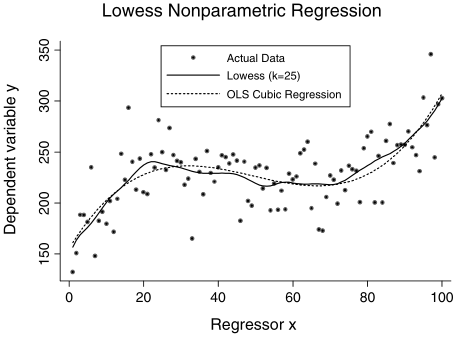
\includegraphics[width=\textwidth]{./resources/CTlowess}
  \label{loclinear2}
  \end{center}
  \end{figure}
\end{frame}

\begin{frame}
\begin{figure}[htbp]
\begin{center}

\includegraphics[width=\textwidth]{./resources/MSTAbstract}
\label{loclinear2}
\end{center}
\end{figure}
\end{frame}

\begin{frame}{Empirical Strategy: DD}
  \begin{figure}[htbp]
  \begin{center}
  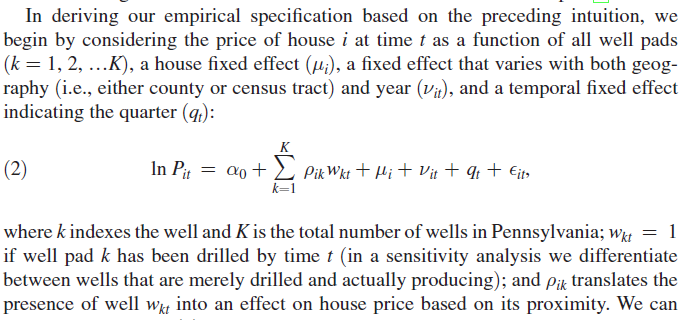
\includegraphics[width=.9\textwidth]{./resources/MSTRegression}
  \label{loclinear2}
  \end{center}
  \end{figure}
\end{frame}

  
\begin{frame}{First show flexible representation}
\begin{figure}[htbp]
\begin{center}
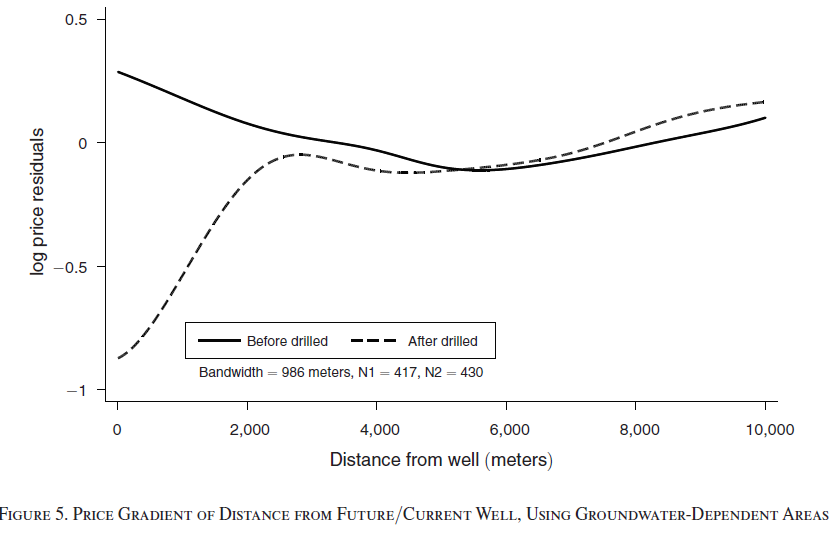
\includegraphics[width=\textwidth]{./resources/MSTGradient}
\label{loclinear2}
\end{center}
\end{figure}
See code in this repo. 
\end{frame}

\frame{\frametitle{Nonparametric Regression, summary, 1}

Nadaraya--Watson for $E(y\vert x)=m(x)$ 
\[
\hat{m}(x)=\frac{\sum_i y_iK_h(x-x_i)}{\sum_i K_h(x-x_i)}
\]
\begin{itemize}
\item bias in $O(h^2)$, variance in $1/(nh^{p_x})$  
\item optimal $h$ in
$n^{-1/(p+4)}$: then bias, standard error and RMSE all converge at
rate $n^{-2/(p+4)}$
\item to select $h$, no rule of thumb: cross-validate on a subsample and
scale up.
\end{itemize}

}

\frame{\frametitle{Nonparametric Regression, summary, 2}

Nadaraya--Watson=\textbf{local constant regression}:  to get $\hat{m}(x)$,

\begin{enumerate}
  \item  regress $y_i$ on $1$ with weight $K_h(x-x_i)$
\item take the estimated coeff as your $\hat{m}(x)$.
\end{enumerate}


\pause

Better: \textbf{local linear regression}

\begin{enumerate}
  \item  regress $y_i$ on $1$ and $(x_i-x)$ with weight $K_h(x-x_i)$
\item take the estimated coeffs as your $\hat{m}(x)$ and $\hat{m}^\prime(x)$.
\end{enumerate}

\pause

To estimate the standard errors: bootstrap on an \emph{undersmoothed}
estimate (so that bias is negligible.)
}

\section{Bootstrap}

\begin{frame}{Bootstrap and Delta Method}
  \begin{itemize}
  \item We know how to construct confidence intervals for parameter estimates:  $\hat{\theta}_k \pm 1.96 SE(\hat{\theta}_k)$
  \item Often we are asked to construct standard errors or confidence intervals around model outputs that are not just parameter estimates: ie:  $g(x_i,\hat{\theta})$.
  \item Sometimes we can't even write $g(x_i,\theta)$ as an explicit function of $\theta$ ie: $\Psi(g(x_i,\theta),\theta) = 0$.
  \item Two options:
  \begin{enumerate}
  \item Delta Method
  \item Bootstrap
  \end{enumerate}
  \end{itemize}
\end{frame}
  
\begin{frame}{Delta Method}
  Delta method works by considering a \alert{Taylor Expansion} of $g(x_i,\theta)$.
  \begin{eqnarray*}
  g(z) \approx g(z_0) + g'(z_0)(z-z_0) + o(||z-z_0||)
  \end{eqnarray*}
  Assume that $\theta_n$ is asymptotically normally distributed so that:
  \begin{eqnarray*}
  \sqrt{n} (\theta_n - \theta_0) \sim N(0,\Sigma)
  \end{eqnarray*}
 % (How do we get this: OLS? GMM? MLE?).\\
  
  Then we have that 
  \begin{eqnarray*}
  \sqrt{n} (g(\theta_n) - g(\theta_0)) \sim N(0,D(\theta)' \Sigma  D(\theta))
  \end{eqnarray*}
  Where $D(\theta) = \frac{\partial g(x_i, \theta)}{\partial \theta}$ is the Jacobian of $g$ with respect to theta evaluated at $\theta$.\\
  We need $g$ to be continuously differentiable around the center of our expansion $\theta$.
\end{frame}
  
  
\begin{frame}{Delta Method: Examples}
  Start with something simple: $Y= \overline{X}_1\cdot \overline{X}_2$ with $(X_{1i},X_{2i}) \sim IID$.
  We know the CLT applies so that:
  \begin{eqnarray*}
  \sqrt{n}
  \begin{pmatrix}
  \overline{X}_1 - \mu_1\\
  \overline{X}_2 - \mu_2
  \end{pmatrix} &\sim  N
  \begin{bmatrix}
  \begin{pmatrix}
  0\\
  0
  \end{pmatrix},
  \Sigma
  \end{bmatrix}
  \end{eqnarray*}
  The Jacobian is just $D(\theta) =  \begin{pmatrix}\frac{\partial g(\theta)}{\partial \theta_1} \\ \frac{\partial g(\theta)}{\partial \theta_2}  \end{pmatrix} =  \begin{pmatrix}\mu_2\\ \mu_1 \end{pmatrix}$\\
  So,
  \begin{eqnarray*}
  V(Y) = D(\theta)' \Sigma D(\theta) =\begin{pmatrix} \mu_2 & \mu_1 \end{pmatrix}  \begin{pmatrix} \sigma_{11} & \sigma_{12} \\ \sigma_{21} & \sigma_{22} \end{pmatrix} \begin{pmatrix} \mu_2 \\\mu_1  
  \end{pmatrix} \\
  \sqrt{n} ( \overline{X}_1 \overline{X}_2 - \mu_1 \mu_2) \sim N(0,\mu_2^2 \sigma_{11}^2 + 2 \mu_1 \mu_2 \sigma_{12}  + \mu_1^2 \sigma_{22}^2)
  \end{eqnarray*}
\end{frame}
  
\begin{frame}{Delta Method: Logit}
  Think about a simple logit:
  \begin{eqnarray*}
  P(Y_i=1 | X_i ) = \frac{\exp^{\beta_0 + \beta_1 X_i}}{1+\exp^{\beta_0 + \beta_1 X_i}} \\
  P(Y_i=0 | X_i ) = \frac{1}{1+\exp^{\beta_0 + \beta_1 X_i}} 
  \end{eqnarray*}
  Remember the ``trick'' to use GLM (log-odds):
  \begin{eqnarray*}
  \log P(Y_i=1 | X_i) - \log P(Y_i=0 | X_i) = \beta_0 + \beta_1 X_i
  \end{eqnarray*}
  \vspace{-10pt}
  \begin{itemize}
  \item Suppose that we have estimated $\hat{\beta_0},\hat{\beta_1}$ via GLM/MLE but we want to know the confidence interval for the probability: $P(Y_i=1 | X_i,\hat{\theta})$
  \item The derivatives are a little bit tricky, but the idea is the same.
  \item This is what STATA should be doing when you type: \tt{mfx, compute}
  \end{itemize}
\end{frame}

%https://faculty.washington.edu/ezivot/econ583/asymptoticsprimerslides.pdf

\begin{frame}{Delta Method: Learning example}
  Often we have a nonlinear model that we transform and estimate linearly.
   
  Here is an example on learning curves from Eric Zivot. 
  \vspace{-15pt}

  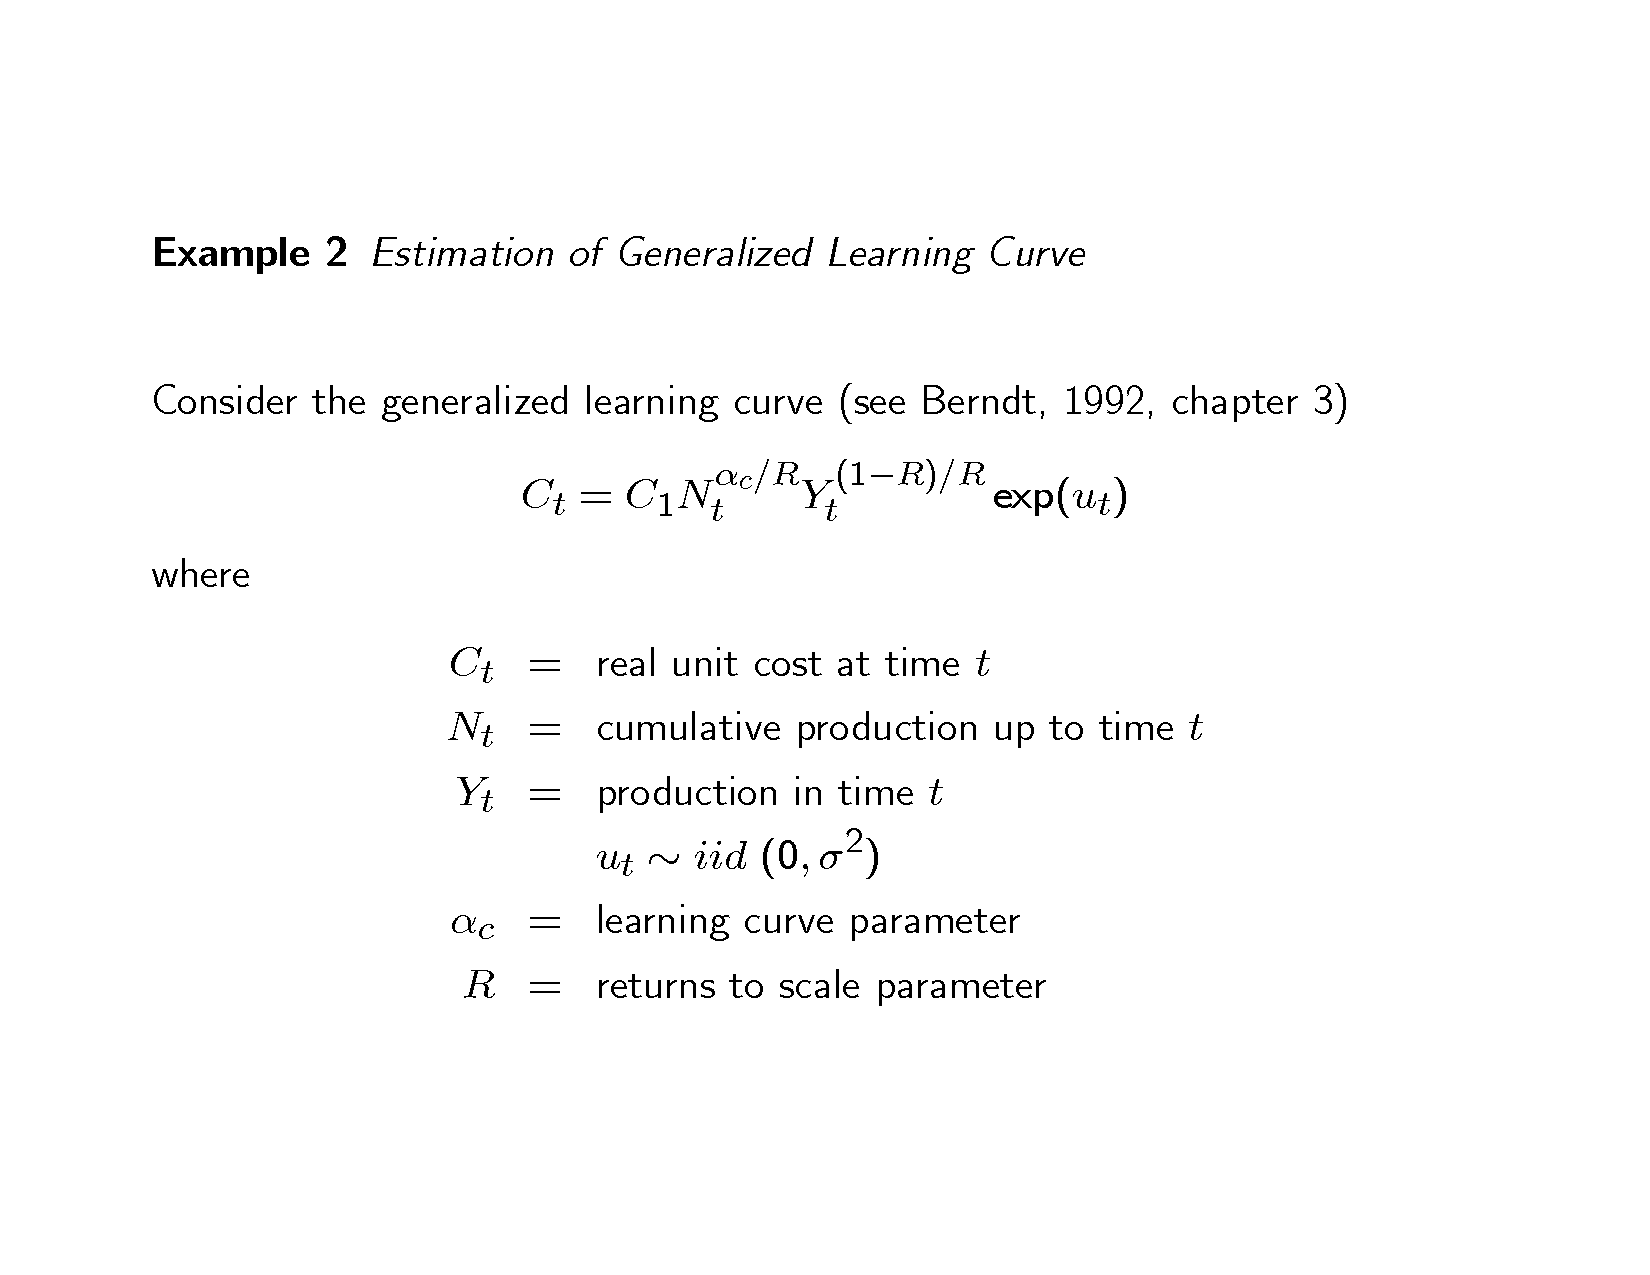
\includegraphics[page=1,trim={2cm 2cm 2cm 2cm},clip,width=\textwidth]{./resources/zivotLearning.pdf}

\end{frame}

\begin{frame}[plain]{}
	\includegraphics[page=2,trim={2cm 2cm 2cm 2cm},clip,width=\textwidth]{./resources/zivotLearning.pdf}
\end{frame}

\begin{frame}[plain]{}
	\includegraphics[page=3,trim={2cm 2cm 2cm 2cm},clip,width=\textwidth]{./resources/zivotLearning.pdf}
\end{frame}

\begin{frame}[plain]{}
	\includegraphics[page=4,trim={2cm 2cm 2cm 2cm},clip,width=\textwidth]{./resources/zivotLearning.pdf}
\end{frame}

\begin{frame}[plain]{}
	\includegraphics[page=5,trim={2cm 2cm 2cm 2cm},clip,width=\textwidth]{./resources/zivotLearning.pdf}
\end{frame}

\begin{frame}[plain]{}
	\includegraphics[page=6,trim={2cm 2cm 2cm 2cm},clip,width=\textwidth]{./resources/zivotLearning.pdf}
\end{frame}

\begin{frame}{Delta Method: Some Failures}
  But we need to be careful.  Suppose that $\theta \approx 0$ and 
  \begin{itemize}
  \item $g(x)  = |X|$
  \item $g(x)  = 1/X$
  \item $g(x)  = \sqrt{X}$
  \end{itemize}
  These situations can arise in practice when we have weak instruments or other problems.\end{frame}
  
\begin{frame}[allowframebreaks]{Bootstrap}
\vspace{-10pt}
  \begin{itemize}
  \item Bootstrap takes a different approach.
  \begin{itemize}
  \item Instead of estimating $\hat{\theta}$ and then using a first-order Taylor Approximation...
  \item What if we directly tried to construct the \alert{sampling distribution} of $\hat{\theta}$?
  \end{itemize}
  
\framebreak
 
  \item Data $(X_1,\ldots,X_n) \sim P$ are drawn from some measure $P$
  \begin{itemize}
  \item We can form a \alert{nonparametric estimate} $\hat{P}$ by just assuming that each $X_i$ has weight $\frac{1}{n}$.
  \end{itemize}
  \item We can then simulate a new sample $X^{*} = (X_1^{*},\ldots X_n^{*}) \sim \hat{P}$.
  \begin{itemize}
  \item Easy: we take our data and construct $n$ observations by \alert{sampling with replacement} 
  \end{itemize}
  \item Compute whatever statistic of $X^{*}$, $S(X^*)$ we would like.
  \begin{itemize}
  \item Could be the OLS coefficients $\beta_1^{*},\ldots, \beta_k^{*}$.
  \item Or some function $\beta_1^{*}/\beta_2^{*}$.
  \item Or something really complicated: estimate parameters of a game $\hat{\theta}^*$ and now find Nash Equilibrium of the game $S(X^{*},\hat{\theta^*})$ changes.
  \end{itemize}
  \item Do this $B$ times and calculate at $Var(S_b)$ or $CI(S_1,\ldots, S_b)$.
  \end{itemize}
\end{frame}
  
\begin{frame}{Bootstrap: OLS}
 \begin{itemize}
 	\item Linear predictor $\beta = E[X_i X_i']^{-1}E[X_i Y_i] $
 	\item Sample $\{(Y_i,X_i) \}_{i=1}^{N}$  
 	\item OLS: $\hat \beta_{ols} = [\sum^N_{i=1} X_i X_i']^{-1}[\sum^N_{i=1} X_i Y_i] $
 	\item To get the variance, resample with replacement B times and calculate $\hat\beta_{ols,b}=   [\sum^N_{j=1} X_j X_j']^{-1}[\sum^N_{j=1} X_j Y_j] $
 	\item Now an estimate of the variance is just 
 	$$ V(\beta_{ols}) = \frac{1}{B}\sum_b^B (\hat \beta_{ols,b} - \bar \beta_{ols,b}) \cdot  (\hat \beta_{ols,b} - \bar \beta_{ols,b})' $$
 \end{itemize}
\end{frame}

\begin{frame}[allowframebreaks]{Bootstrap: Variants}
  The bootstrap I have presented is sometimes known as the \alert{nonparametric bootstrap} and is the most common one.
  \begin{description}
  \item[Parametric Bootstrap] instead of bootstrapping pairs $(Y_i,X_i)$, we can bootstrap the residuals. 
  \begin{itemize}
  	\item First estimate $\hat \beta_{ols}$ by OLS
  	\item Get residuals $\hat \epsilon_i = Y_i - X_i'\hat{\beta_{ols}}$ 
  	\item For $b=1,...,B$, resample $N$ residuals $\hat \epsilon_i$
  	\item Predict a new $Y_{b,j} = X_j' \hat \beta_{ols} + \hat \epsilon_{b,j}$
  	\item Estimate with OLS and proceed as before. 
  \end{itemize}
\framebreak

   \item[Wild Bootstrap] Similar to parametric bootstrap but we rescale $\epsilon_i$ to allow for \alert{heteroskedasticity}
  \item[Block Bootstrap] For correlated data (e.g.: time series). Blocks can be overlapping or not.  
  \end{description}
\end{frame}
  
\begin{frame}{Bootstrap: Bias Correction}
  \small
  The main idea is that $\hat{\theta}^{1*},\ldots, \hat{\theta}^{B*}$ approximates the \alert{sampling distribution} of $\hat{\theta}$. There are lots of things we can do now:
  \begin{itemize}
  \item We already saw how to calculate $Var(\hat{\theta}^{1*},\ldots, \hat{\theta}^{B*})$.
  \begin{eqnarray*}
  \frac{1}{B-1} \sum_{b=1}^B (\hat{\theta}_{(b)}^* - \overline{\theta^{*}})^2
  \end{eqnarray*}
  
  \item Calculate $E(\hat{\theta}^{*}_{(1)},\ldots, \hat{\theta}^{*}_{(B)}) = \overline{\theta^{*}} = \frac{1}{B} \sum_{b=1}^B \hat{\theta}_{(b)}^*$.
  \begin{itemize}
  \item We can use the estimated bias to \alert{bias correct} our estimates
  \begin{eqnarray*}
  Bias(\hat{\theta}) &=&E[\hat{\theta}] - \theta \\
  Bias_{bs}(\hat{\theta}) &=&\overline{\theta^{*}} -\hat{\theta}
  \end{eqnarray*}
  Recall $\theta = E[\hat{\theta}] - Bias[\hat{\theta}]$:
  \begin{eqnarray*}
  \hat{\theta}- Bias_{bs}(\hat{\theta}) = \hat{\theta}-(\overline{\theta^{*}}-\hat{\theta}) = 2 \hat{\theta} - \overline{\theta^{*}}
  \end{eqnarray*}
  \end{itemize}
  \item Correcting bias isn't for free - variance tradeoff!
  \item Linear models are (hopefully) unbiased, but most nonlinear models are \alert{consistent but biased}.
  \end{itemize}
  \end{frame}
  
  
\begin{frame}{Bootstrap: Confidence Intervals}
  There are actually three ways to construct bootstrap CI's:
  \begin{enumerate}
  \item Obvious way: sort  $\hat{\theta}^{*}$ then take $CI: [\hat{\theta}^{*}_{\alpha/2},\hat{\theta}^{*}_{1-\alpha/2}]$.
  \item Asymptotic Normal:  $CI: \hat{\theta} \pm 1.96 \sqrt{V(\hat{\theta}^{*})}$. (CLT).
  \item Better Way: Use a pivotal statistic that you know the distribution of.
  \end{enumerate}
\end{frame}

\begin{frame}{Bootstrap CI: percentile t method}
  \begin{itemize}
    \item Instead of estimating $\theta_b$ for each bootstrap sample, estimate the t-statistic $t^b = (\hat \theta^b - \hat \theta )/ s_{\hat \theta^b \theta}$, where $\hat \theta$ is the original estimate. 
    \item The empirical distribution of $t^b$ can then be used to approximate the \textbf{known} t-distribution (which has nothing to do with our data)
    \item Let $t^b_{[1-\alpha/2]}$ and $t^b_{[\alpha/2]}$ denote the lower and upper $\alpha/2$ quintiles of this distribution. 
    \item A confidence interval can then be constructed as 
    $$ \left( \hat \theta - t^b_{[1-\alpha/2]} \times \hat s_{\hat \theta}, \hat \theta + t^b_{[\alpha/2]} \times \hat s_{\hat \theta} \right) $$
  \end{itemize}
\end{frame}
  
\begin{frame}{Bootstrap: Why do people like it?}
  \begin{itemize}
  \item Econometricians like the bootstrap because under certain conditions it is \alert{higher order efficient} for the confidence interval construction (but not the standard errors).
  \begin{itemize}
  \item Intuition: because it is non-parametric it is able to deal with more than just the first term in the Taylor Expansion (actually an \alert{Edgeworth Expansion}).
  \item Higher-order asymptotic theory is best left for real econometricians!
  \end{itemize}
  \item Practitioner's like the bootstrap because it is easy.
  \begin{itemize}
  \item If you can estimate your model once in a reasonable amount of time, then you can construct confidence intervals for most parameters and model predictions.
  \end{itemize}
  \end{itemize}
  \end{frame}
  
  \begin{frame}{Bootstrap: When Does It Fail?}
  \begin{itemize}
  \item Bootstrap isn't magic. If you are constructing standard errors for something that isn't asymptotically normal, don't expect it to work!
  \item The Bootstrap exploits the notion that your sample is IID (by sampling with replacement). If IID does not hold, the bootstrap may fail (but we can sometimes fix it!).
  \item Bootstrap depends on asymptotic theory. In small samples weird things can happen. We need $\hat{P}$ to be a good approximation to the true $P$ (nothing missing).
  \end{itemize}
  \end{frame}
  
  
\begin{frame}{Bootstrap vs Delta Method}
  \begin{itemize}
  \item Delta Method works best when working out Jacobian $D(\theta)$ is easy and statistic is well approximated with a linear function (not too curvy).
  \item I would almost always advise Bootstrap unless:
  \begin{itemize}
  \item Delta method is trivial e.g.: $\beta_1 / \beta_2$ in linear regression.
  \item Computing model takes many days so that 10,000 repetitions would be impossible.
  \end{itemize}
  \item Worst case scenario: rent time on Amazon EC2!
  \begin{itemize}
  \item I ``bought'' over \$1,000 of standard errors recently.
  \end{itemize}
  \item But neither is magic and both can fail!
  \end{itemize}
\end{frame}

% from CT 9.5.4
\begin{frame}{CI's for Kernel Smoothers}
  \begin{itemize}
    \item Return to the theme of these slides: Estimating a nonparametric regression function. 
    \item For kernel regression, you need to present CI's \textbf{pointwise}. 
    \begin{itemize}
      \item CT recommend presenting CIs for $f(x_0)$ for the first nine deciles of $x$
    \end{itemize}

\pause

    \item If we ignore the bias $b(x_0)$ inherent in $\hat m(x_0)$ then, 
    $$ m(x_0) \in \hat m(x_0) \pm 1.96 \sqrt{\frac{1}{Nh}{\hat \sigma_\epsilon^2}{\hat f(x_0)} \int K(z)^2dz} $$
    where $\hat \sigma_\epsilon^2 = \sum_i w_{i0,h}\hat \epsilon^2$ and $\hat f(x_0)$ is the kernel density estimate at $x_0$
    \item Since we know that there is bias, if we use $h_{opt}$, this CI will suffer from \textbf{undercoverage}
    \item On option is to undersmooth. By pick a bigger $h$, the bias goes to zero, the square of the bias will converge faster than the variance 
  % see guido's notes 17 for this
  \end{itemize}
\end{frame}

% from CT 9.5.4
\begin{frame}{An alternative is to bootstramp CI's}
  Consider the following routine proposed by Yatchew. 
  \begin{enumerate}
    \item Use CV to find the optimal bandwith. Call this $\lambda$ and the estimated function $f_\lambda$
    \item Reestimate $f$ with using a \textit{wider} bandwidth $\bar \lambda = 1.1 \lambda$ (oversmoothing)
    \item Reestimate $f$ with using a \textit{narrower} bandwidth of $.9 \lambda$. Get \textit{undersmoothed} residuals $\hat \epsilon_i$
    \item Center residuals and use \textbf{parametric} boostrap to generated $B$ samples $y_i^b = \hat f_{\bar \lambda}(x_i) + \hat \epsilon_i^b$
    \item Now estimate $\hat f_\lambda^b(x_0)$ using the \textbf{original} $\lambda$
    \item Can obtain 95\% CIs from 0.025 and 0.975 quintiles of $\hat f^B_{\lambda}(x_0)$
  \end{enumerate}
\end{frame}

\section{Basis Expansions}

\begin{frame}{Seminonparametric (=Flexible) Regression}
  \begin{itemize}
    \item Linear model won't fit well when true relationship is nonlinear
    \item But fully flexible models may require a lot of data 
    \item Alternative is to replace $X$ with $M$ transformations of $h_m(X)$
    \item Then model $f(X) = \sum_m \beta_m h_m(X)$
  \end{itemize}
\end{frame}

\begin{frame}{Series or sieves}

  \begin{itemize}
    \item This is a \textit{parametric} approximation that becomes more accurate as the sample size increases
  
    \item {\bf Idea:} we add regressors when we have more data, eventually providing an arbitrarily close approximation to the true regression function
  
    \item Polynomial Example: $ m(x;\beta_K) = \sum_{j=1}^{K} \hat \beta_j x^j$ 
    \item Given $K$, \textbf{just estimate model using OLS}
    \item In practice, you'll want to choose $K$ using leave-one-out cross validation. 
  \end{itemize}
  
  Note that simply polynomials often perform poorly in some parts of the data! 
  
\end{frame}

\begin{frame}
  \frametitle{Piecewise polynomials}
  \begin{itemize}
    \item First consider a single dimensional $X$
    \item Divide $f$ into contiguous intervals, and pick a function to represent $y$ on each interval 
    \item A natural starting point would be a piecewise constant function, broken up by boundary points $\xi_1$ and $xi_2$
    $$ h_1 = I(X < \xi_1) ; h_2 = I(\xi_1 < X < \xi_2); h_3 = I(\xi_2 < X) $$ 
    \item This predicts the interval average for all $X$

  \end{itemize}
\end{frame}    

\begin{frame}
  \begin{figure}[htbp]
  \begin{center}
  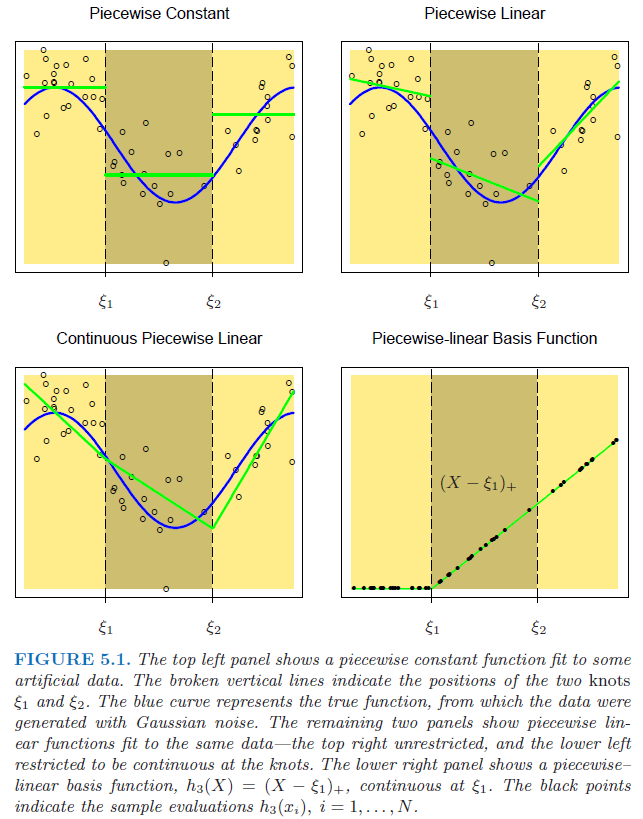
\includegraphics[height=\textheight]{./resources/ESLPiecewise}
  \end{center}
  \end{figure}
\end{frame}

\begin{frame}
  \frametitle{Piecewise polynomials (cont)}
  \begin{itemize}
     \item We can improve this by adding three additional basis functions: $h_{m+3} = h_m(X)X$. 
    \item We can then make it continuous by 
    \begin{eqnarray*}
      h_1 = 1 \\
      h_2 = X \\
      h_3 = (X- \xi_1)_+ \\
      h_4 = (X - \xi_2)_+ 
    \end{eqnarray*} 
  \end{itemize}
\end{frame}

\begin{frame}
  \frametitle{Smooth splines}
  \begin{itemize}
    \item We can improve this further by increasing the order of the local polynomial
    \item A common option is cubic splines: 
    \begin{eqnarray*}
      h_1 = 1  ; \quad  h_2 = X  ; \quad h_3 = X^2 \\
      h_4 = x^ 3  ; \quad h_5 (X- \xi_1)_+^3 ; \quad h_6 = (X - \xi_2)_+^3 
    \end{eqnarray*} 
    \item This is a six dimensional space: (3 regions) X (4 parameters per region) - (2 knots) X (3 constraints per knot)
    \item In practice people never use higher than cubic
    \item Picking the knots is more subjective (use CV?)
    \item Also typically use B-splines (see HTF)
  \end{itemize}

 \end{frame}

 
\begin{frame}
  \begin{figure}[htbp]
  \begin{center}
  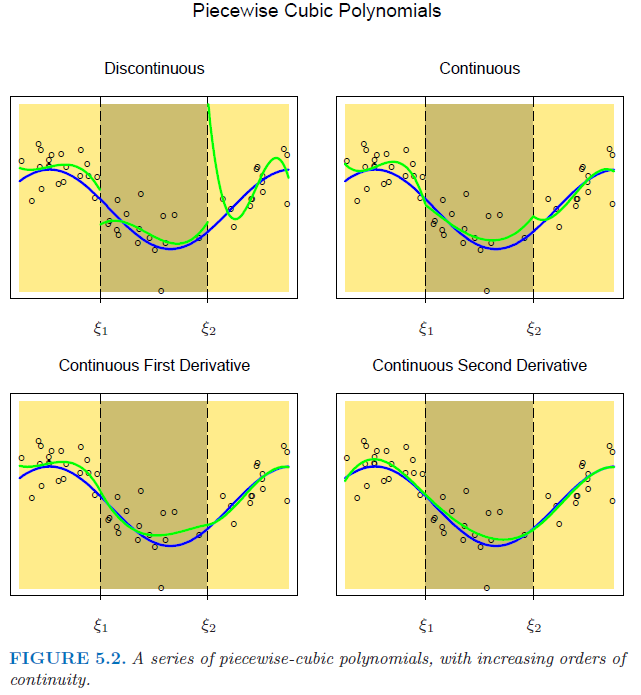
\includegraphics[height=\textheight]{./resources/ESLPiecewiseCubic}
  \end{center}
  \end{figure}
\end{frame}

\begin{frame}{Natural Splines}
  THF: "We know that the behavior of polynomials fit to data tends to be erratic
  near the boundaries, and extrapolation can be dangerous. The polynomials fit beyond the boundary knots behave even more wildly than the corresponding global polynomials
  in that region." 

  \alert{Natural Cubic Splines} Add a further constraint that the fitted function is linear beyond the boundary knots

  With K knots is represented by K basis functions:
\vspace{-8pt}
  \begin{eqnarray*}
    h_1 = 1 \\
    h_2 = X \\
    h_{k+2} = d_k - d_{K-1}
  \end{eqnarray*} 
  where, $$d_k(X) = \frac{(X-\xi_k)_+^3 - (X-\xi_k)_+^3 }{\xi_K - \xi_k} $$
\end{frame}


\begin{frame}{Smoothing Splines}
Idea: pick knots to minimize RSS 

\[
\min_{m(.)} \sum_i^N (y_i-f(x_i))^2 +\lambda J \int (f''(x))^2 dx 
\]

where $\lambda$ is a \textbf{smoothing parameter} and $f(x)$ is any twice differentiable function

Remarkably, THF show that the solution can be represented as a natural cubic spline with knots at $k$ chosen points. 

We'll discuss this \alert{shrinkage} estimator next week.
\end{frame}

\begin{comment}
\begin{frame}{Series or sieves}

\begin{itemize}
  \item This is a \textit{parametric} approximation that becomes more accurate as the sample size increases

  \item {\bf Idea:} we add regressors when we have more data, eventually providing an arbitrarily close approximation to the true regression function

  \item Polynomial Example: $ m(x;\beta_K) = \sum_{j=1}^{K} \hat \beta_j x^j$ 
  \item Given $K$, \textbf{just estimate model using OLS}
  \item In practice, you'll want to choose $K$ using leave-one-out cross validation. 
\end{itemize}

Note that simply polynomials often perform poorly in some parts of the data! 

\end{frame}


\begin{frame}{Splines: trading off fit and smoothness}

  \begin{itemize}
    \item Another option is to use splines
    \item {\bf Idea:} Approximate regression function \textit{locally} using (low order) polynomials, then connect these polynomials at knots. 
    \item The regression function will be continuous at the knots, but not as many times differentiable as elsewhere
    \item For example, can estimate a linear spline with an intercept and separate slopes depending on whether $x > x_0$
  \end{itemize}
\end{frame} 
\end{comment}

%
\section{Semi-parametrics}

\begin{frame}{Semiparametric Regression}
  \begin{itemize}
    \item Previous methods placed no structure on the model
    \item Sometime we're willing to impose \textit{some} structure, typically to isolate a parameter or ratio that we're particularly interested in
    \item Fully non-parametric methods controlling for other factors not possible due to the curse of dimensionality. 
  \end{itemize}
\end{frame}

\begin{frame}
  \frametitle{Examples}
  
  \begin{figure}[htbp]
    \begin{center}
    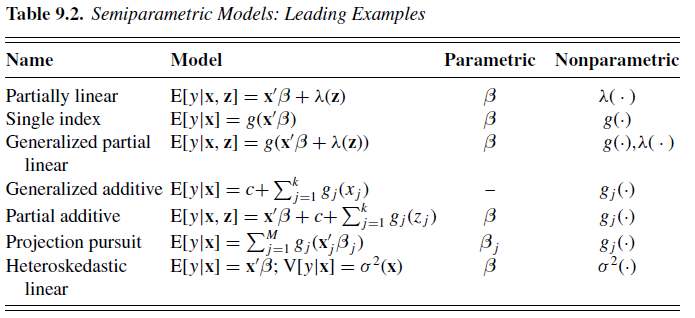
\includegraphics[width=\textwidth]{./resources/CTSemiPExamples}
    \label{loclinear2}
    \end{center}
  \end{figure}

  For a formal treatment of these and discussion of convergence, see \cite{powell_chapter_1994}.
\end{frame}

\begin{frame}
  \frametitle{Partial linear model}
  We'll focus on the most commonly used model: the \textbf{partial linear model} 
  $$ y_i = X_i'\beta + g(Z_i) + e_i $$ 
  
  We are interested in $\beta$, but $g()$ is an unrestricted (unknown) function of $z$. 

  Identification requires $Cov[X,g(Z)]=0$ 

  \citet{robinson_root-n-consistent_1988} showed that we can concentrate this $g()$ out of the model. 

\end{frame}

\begin{frame}[allowframebreaks]
  \frametitle{Robinson 1988}
  $$ y_i = X_i'\beta + g(Z_i) + e_i $$ 
  where $e_i = y_i - E[y_i | X_i,Z_i]$. 
  
  Take the conditional expectation
  $$ E[y_i | Z_i]  = E [X_i | Z_i]'\beta + g(Z_i) + E[e_i | Z_i] $$ 
  then note that $E[e_i | Z_i] = E[E[e_i | X_i,Z_i]] = 0$ 

  Subtractcing yields 

  $$ y_i - E[y_i | Z_i] = (X_i - E [X_i | Z_i])'\beta + e_i $$

  \framebreak 

  So this suggests a natural procedure: 

  1. Estimate the conditional expectations $m_y(z) = E[y_i | Z_i]$ and $m_x(z) = E[X_i | Z_i]$ separately (and flexibly) \textbf{for each $x$} using the methods discussed in the previous section. 

  2. Estimate $\beta$ using OLS on the residuals 
  
  $$y_i - \hat m_y(z_i) =  (X_i - \hat m_x(z_i))'\beta + e_i $$

  \pause 

  Note: Yatchew (1997) suggest step 1 can be avoided entirely by simply sorting on $z$, and running the model in first-differences. 

  For a recent example, Hastings and Shapiro (AER 2018)
\end{frame}

\begin{frame}[allowframebreaks]{Single-Index Models}
   
  \begin{itemize}
  \item Assume we are willing to specify that the conditional mean is a scalar function of the linear combination of $X's$ 
  $$ E \left[ y | \mathbf{x} \right] = g(\mathbf{x}'\beta ) $$ 
  \item Often we'll assume $g()$ as in logit and probit. 
  \item Instead, note that the conditional mean of a change in $x$ 
  $$ \delta \equiv E \left[g'(\mathbf{x}'\beta ) \beta_j \right] $$ 
  
  \item Suggests the \alert{average derivative estimator} which doesn't require normality assumptions of probit
  \item Let $m(x_i) = g(x_i'\beta)$. 
  $$ \hat \delta_{AD} = -\frac{1}{N} \sum_{i=1}^N y_i \frac{f'(x_i)}{f(x_i)} $$
  where $f(x)$ is the density of $x$

  \item More robust, but potentially less efficient if true distribution of $\varepsilon \sim N(0,1)$.
 
  \item Can use Marginal Rate of Substitution (MRS) to identify $\beta_k / \beta_l$.
  $$ \frac{ \partial \left[ y | \mathbf{x} \right] / \partial x_j }{ \partial \left[ y | \mathbf{x} \right] / \partial x_k} = \frac{\beta_j}{\beta_k} $$ 
  
   \end{itemize}
\end{frame}

\begin{frame}{Review: What was the point?}
  \begin{itemize}
  \item OLS is lowest variance among linear unbiased estimators.
  \item But there are \alert{nonlinear} estimators and potentially \alert{biased} estimators.
  \begin{itemize}
  \item Everything faces a \alert{bias-variance} tradeoff.
  \item Nearly anything can be written as Kernel.
  \end{itemize}
  \end{itemize}

\end{frame}

%%%%%%%%%%%%%%%%%%%%%%%%%%%%%%%%%%%%%%%%%%%%%%%%%%%%%%%%%%%%%%%%%%%%%%
\begin{frame}[allowframebreaks]
  \bibliographystyle{jpe}
  \bibliography{../empirical-methods}
\end{frame}

\end{document}

%\begin{frame}
%\frametitle{Additive models}
%\pause
%{\em Additive model:} $y=\alpha+\sum_{j=1}^p + f_j (X_j) + +\epsilon$\\
%\pause
%{\em Backfitting algorithm:} start with $\hat{a}=\overline{y}_n$, and some zero--mean
%guesses  $\hat{f}_j \equiv 0 $.
%\pause
%Then for $j=1,\ldots,p,\ldots ,1,2,\ldots,p,\ldots$,
%\pause
%\begin{enumerate}[<+->]
%\item   Define 
%\begin{eqnarray*}
%f_j &\leftarrow& S_j[\{y_i - \hat{\alpha} - \sum_{k\neq j} \hat{f}_k (x_{ik})\}_1^N ]\\
%f_j &\leftarrow&  \hat{f}_j - \frac{1}{N} \sum_{i=1}^N \hat{f}_j (x_{ij}).
%\end{eqnarray*}
%\item Regress $\hat{y}$ on $x_j$ to get $R_j$; then replace $\hat{r}_j$ with $R_j-\frac{1}{n}\sum_i \hat{r}_j(x_{ji})$ (where $S_j$ is some cubic smoothing spline).
%\item Iterate until $\hat{f}_j$ doesn't change.
%\end{enumerate}
%\end{frame}
%



\section*{unused}
%% OLD / UNUSED (BUT USEFUL) SLIDES


% PROBABLY NOT GOING TO USE THE IDENTIFICATION STUFF 
\begin{comment}
  \begin{frame}{Something Familiar}
    Let's start with something we all know, how to calculate:
    \begin{eqnarray*}
    E[Y_i | X_i ] = \beta_0 + \beta_1 X_1 + \ldots + \varepsilon_i
    \end{eqnarray*}
    \begin{itemize}
    \item The Gauss-Markov theorem (remember that?) tells us that OLS is best among linear unbiased estimators.
    \end{itemize}
  \end{frame}
  
  \begin{frame}{Identification}
    What does it mean for a model to be identified?
    \begin{eqnarray*}
    \hat{\beta}_{OLS} = \arg \max_{\beta} (\mathbf{y} - \mathbf{x} \beta)' (\mathbf{y} - \mathbf{x} \beta)
    \end{eqnarray*}
    \begin{itemize}
    \item We need there to be a unique value of $\beta$ that solves the above equation.
    \item For OLS this reduces to solving a linear system of $\dim(X)=k$ equations and unknowns.
    \item The OLS estimator produces $\hat{\beta}_{OLS} = \beta + (X'X)^{-1}X'\varepsilon$.
    \begin{itemize}
    \item Identification: means that we require $(X'X)$ is invertible (no perfect multicollinearity).
    \item When $E[X' \varepsilon ] =0$ then this converges in probability to true $\beta$.
    \end{itemize}
  
    \end{itemize}
  \end{frame}
  
  \begin{frame}{A Little More Complicated}
  \begin{itemize}
  \item For many cases that we care about, $E[X' \varepsilon ] \neq 0$. (Endogeneity)
  \item We know this is not the end of the world if we have an instrument $Z$:
  \item Now we need that $Z'X$ is invertible.
  \end{itemize}
  \begin{eqnarray*}
  E[\mathbf{x}' (\mathbf{y} - \mathbf{x} \beta)] &\neq& 0\\
  E[\mathbf{z}' (\mathbf{y} - \mathbf{x} \beta)] &=&0\\
  \rightarrow \hat{\beta}_{TSLS} &=& E(Z'X)^{-1} E[Z'Y]
  \end{eqnarray*}
  \end{frame}
  
  
  \begin{frame}{Some more information}
  This leads to the common terminology:
  \begin{itemize}
  \item Under-identified: if $\dim(X) > \dim(Z)$.
  \item Just-identified: if $\dim(X) = \dim(Z)$.
  \item Over-identified: if $\dim(X) < \dim(Z)$.
  \end{itemize}
  \end{frame}
  
  \begin{frame}{What does this mean exactly}
  To understand this we usually construct the GMM form of the moment conditions:
  \begin{eqnarray*}
  E[\mathbf{z}' (\mathbf{y} - \mathbf{x} \beta)] &=&0\\
  f(\beta)&=&  (\mathbf{y} - \mathbf{x} \beta)' \mathbf{z} \cdot W \cdot \mathbf{z}' (\mathbf{y} - \mathbf{x} \beta)
  \end{eqnarray*}
  \begin{itemize}
  \item Because $f(\beta)$ is a quadratic form, and when $W$ is PSD then $f(\beta) \geq 0$.
  \item Just-identified: There is exactly one solution to $f(\beta) = 0$ which does not depend on $W$.
  \item Under-identified: $f(\beta) = 0$ has many solutions because we have fewer instruments (or moment restrictions) than parameters.
  \item Over-identified: There are no solutions and $f(\beta) > 0$. Instead we choose $\beta$ to minimize the distance from zero with distance metric $W$.
  \end{itemize}
  \end{frame}
  
  \begin{frame}{The Binary Case}
  Now let's think about a case where $Y \in \{0,1\}$:
  \begin{eqnarray*}
  y_i = \mathbf{1}[F(X_i) - \varepsilon_i > 0]
  \end{eqnarray*}
  \begin{itemize}
  \item There are different choices of $F(X_i)$ and $f(\varepsilon)$
  \item  Probit: $F(X_i) = \beta X_i$ where $\varepsilon_i \sim N(0,1)$.
  \item  Logit: same $F(\cdot)$ but different $f(\varepsilon)$ (Type I Extreme Value). $P(Y_i = 1 | X_i) = 1/(1+exp[-\beta X_i])$.
  \item These choices of $F$ are strong and somewhat arbitrary, we choose them out of convenience because both transformations are monotonic in $\beta X_i$, and continuously map $[-\infty,\infty] \rightarrow [0,1]$
  \end{itemize}
  \end{frame}
  
  \begin{frame}{The Binary Case}
  What is the least I can assume in the binary case and still learn something?
  \begin{eqnarray*}
  y_i = \mathbf{1}[F(X_i) - \varepsilon_i > 0]
  \end{eqnarray*}
  \begin{itemize}
  \item Suppose instead we observe $P(x) = Pr(y_i = 1 | x_i)$ at many values of $x_i$. (Often refer to this as the CCP).
  \item Sometimes CCPs are all we care about. (if we are lucky).
  \end{itemize}
  Instead we can try and solve:
  \begin{eqnarray*}
  P(x) = \int \mathbf{1}(F(x) - \varepsilon > 0) dH(\varepsilon | x) = H(F(x)| x)
  \end{eqnarray*}
  \begin{itemize}
  \item Identification asks, what is the least we need to assume in order to recover $F,H$?
  \item Even with $\varepsilon \perp X$ we still have too many degrees of freedom.
  \end{itemize}
  \end{frame}
  
  \begin{frame}{Are we stuck?}
  
  \begin{itemize}
  \item We know that Logit and Probit are identified.
  \item Start with $\varepsilon \perp X$.
  \item $F(X_i) = G(X_i \beta)$ is a very powerful assumption often called \alert{(single) index model}
  \item Can use Marginal Rate of Substitution (MRS) of $P(x)$ to identify $\beta_k / \beta_l$.
  \begin{itemize}
  \item How do conditional probabilities respond to changes in $X^{(k)}$ versus $X^{(l)}$?
  \item Suggests the \alert{average derivative estimator} which doesn't require normality assumptions of probit
  \item More robust, but potentially less efficient if true distribution of $\varepsilon \sim N(0,1)$.
  \end{itemize}
  \item Can we extend the general intuition to more cases?
  \end{itemize}
  \end{frame}
  
  
  \begin{frame}{Single-Index Models}
   
    \begin{itemize}
    \item Consider $$ E \left[ y | \mathbf{x} \right] = g(\mathbf{x}'\beta ) $$ 
    such as logit and probit. 
    \item With conditional mean of change in $x_j$ 
    $$ \frac{ \partial \left[ y | \mathbf{x} \right]}{\partial x_j} = g'(\mathbf{x}'\beta ) \beta_j $$ 
    
    \item Can use Marginal Rate of Substitution (MRS) to identify $\beta_k / \beta_l$.
    $$ \frac{ \partial \left[ y | \mathbf{x} \right] / \partial x_j }{ \partial \left[ y | \mathbf{x} \right] / \partial x_k} = \frac{\beta_j}{\beta_k} $$ 
    
    \item Suggests the \alert{average derivative estimator} which doesn't require normality assumptions of probit
    \item More robust, but potentially less efficient if true distribution of $\varepsilon \sim N(0,1)$.
    \item Can we extend the general intuition to more cases?
    \end{itemize}
  \end{frame}
\end{comment}
  
